\documentclass[11pt,letterpaper]{article}

% ------------------------------------------------------------
%  Packages
% ------------------------------------------------------------
\usepackage[utf8]{inputenc}
\usepackage[margin=1in]{geometry}
\usepackage{amsmath,amssymb,amsthm,mathtools}
\usepackage{booktabs}
\usepackage{enumitem}
\usepackage{titlesec}
\usepackage{xcolor}
\usepackage{etoolbox}
\usepackage{microtype}
\usepackage[skins,breakable]{tcolorbox}
\usepackage[parfill]{parskip}
\usepackage[hidelinks]{hyperref}

\hypersetup{
  pdftitle  = {STAT 110 -- Introduction to Probability},
  pdfauthor = {Obrian Buchanan}
}

% ------------------------------------------------------------
%  Colours (clean, airy, modern)
% ------------------------------------------------------------
\definecolor{ink}{HTML}{1E293B}        % slate-900 (crisp modern charcoal)
\definecolor{textsub}{HTML}{64748B}    % slate-500 (subtle secondary text)

% Light, translucent-style background tints & hairline borders
\definecolor{defshade}{HTML}{F8FAFC}   % slate-50 (ultra-light cool frost)
\definecolor{defborder}{HTML}{E2E8F0}  % slate-200 (hairline border)
\definecolor{thmshade}{HTML}{FBFBF9}   % warm alabaster tint
\definecolor{thmborder}{HTML}{E7E5E4}  % stone-200 (hairline border)
\definecolor{storyshade}{HTML}{F4F7F4} % muted sage tint for probability stories
\definecolor{storyborder}{HTML}{DCE3DC}% soft sage border

% ------------------------------------------------------------
%  Spacing
% ------------------------------------------------------------
\linespread{1.12}
\setlength{\parskip}{0.55em}
\setlength{\jot}{7pt}

\AtBeginDocument{%
  \setlength{\abovedisplayskip}{9pt plus 2pt minus 2pt}%
  \setlength{\belowdisplayskip}{9pt plus 2pt minus 2pt}%
  \setlength{\abovedisplayshortskip}{5pt plus 2pt}%
  \setlength{\belowdisplayshortskip}{7pt plus 2pt}%
}

\setlist{leftmargin=1.8em, topsep=0.5em, itemsep=0.5em, parsep=0.25em}

% Tables and matrices: a little more room between rows and columns
\renewcommand{\arraystretch}{1.15}
\setlength{\arraycolsep}{4pt}

% Grey justification next to a derivation step, e.g. \by{LOTP}
\newcommand{\by}[1]{\text{\small\color{gray!80!black}#1}}

% ------------------------------------------------------------
%  Probability notation
% ------------------------------------------------------------
\newcommand{\E}{\operatorname{E}}           % expectation
\newcommand{\Var}{\operatorname{Var}}       % variance
\newcommand{\Cov}{\operatorname{Cov}}       % covariance
\newcommand{\Corr}{\operatorname{Corr}}     % correlation
\newcommand{\Bern}{\operatorname{Bern}}
\newcommand{\Bin}{\operatorname{Bin}}
\newcommand{\HGeom}{\operatorname{HGeom}}
\newcommand{\Geom}{\operatorname{Geom}}
\newcommand{\NBin}{\operatorname{NBin}}
\newcommand{\FS}{\operatorname{FS}}
\newcommand{\Pois}{\operatorname{Pois}}
\newcommand{\DUnif}{\operatorname{DUnif}}
\newcommand{\Unif}{\operatorname{Unif}}
\newcommand{\Expo}{\operatorname{Expo}}
\newcommand{\Norm}{\mathcal{N}}             % Normal: \Norm(\mu, \sigma^2)
\newcommand{\indep}{\perp\!\!\!\perp}       % independence symbol
\newcommand{\iid}{\overset{\text{i.i.d.}}{\sim}}

% ------------------------------------------------------------
%  Headings
% ------------------------------------------------------------
% Chapter title (section): number hidden in the body, shown in the TOC
\titleformat{\section}
  {\LARGE\bfseries\color{ink}}{}{0em}{}
\titlespacing*{\section}{0pt}{0pt}{2.2em}

% Subsection: numbered so each part is easy to spot
\titleformat{\subsection}
  {\Large\bfseries\color{ink}}{\thesubsection}{0.8em}{}
\titlespacing*{\subsection}{0pt}{2.6em}{1.0em}

% Subsubsection: smaller, unnumbered
\titleformat{\subsubsection}
  {\large\bfseries\color{ink}}{}{0em}{}
\titlespacing*{\subsubsection}{0pt}{1.8em}{0.6em}

\setcounter{tocdepth}{2}

% ------------------------------------------------------------
%  Numbering: one shared counter per chapter (Def 2.1, Thm 2.2, Ex 2.3, ...)
% ------------------------------------------------------------
\newcounter{note}[section]
\renewcommand{\thenote}{\thesection.\arabic{note}}

% ------------------------------------------------------------
%  Box styles (Modern frosted card aesthetic)
% ------------------------------------------------------------
\tcbset{
  notebox/.style={
    enhanced,
    boxrule=0.6pt,
    arc=4pt,
    left=14pt, right=14pt, top=10pt, bottom=10pt,
    before skip=1.5em, after skip=1.5em,
    detach title,
    fonttitle=\bfseries\small, coltitle=ink,
    before upper={\tcbtitle\par\vspace{0.4em}},
    opacityback=0.9
  },
  defbox/.style={
    notebox,
    colback=defshade,
    colframe=defborder
  },
  thmbox/.style={
    notebox,
    colback=thmshade,
    colframe=thmborder
  },
  storybox/.style={
    notebox,
    colback=storyshade,
    colframe=storyborder
  }
}

% Builds the box title, e.g. "Definition 2.1 (Conditional Probability)"
\newcommand{\notetitle}[2]{#1~\thenote\ifstrempty{#2}{}{\ (#2)}}

% Definition: frosted slate card
\NewDocumentEnvironment{definition}{O{}}
  {\refstepcounter{note}\begin{tcolorbox}[defbox, title={\notetitle{Definition}{#1}}]}
  {\end{tcolorbox}}

% Theorem-type results: frosted stone card
\NewDocumentEnvironment{theorem}{O{}}
  {\refstepcounter{note}\begin{tcolorbox}[thmbox, title={\notetitle{Theorem}{#1}}]}
  {\end{tcolorbox}}

\NewDocumentEnvironment{proposition}{O{}}
  {\refstepcounter{note}\begin{tcolorbox}[thmbox, title={\notetitle{Proposition}{#1}}]}
  {\end{tcolorbox}}

\NewDocumentEnvironment{lemma}{O{}}
  {\refstepcounter{note}\begin{tcolorbox}[thmbox, title={\notetitle{Lemma}{#1}}]}
  {\end{tcolorbox}}

\NewDocumentEnvironment{corollary}{O{}}
  {\refstepcounter{note}\begin{tcolorbox}[thmbox, title={\notetitle{Corollary}{#1}}]}
  {\end{tcolorbox}}

% Story: the real-world setup behind a distribution or a counting argument
\NewDocumentEnvironment{story}{O{}}
  {\refstepcounter{note}\begin{tcolorbox}[storybox, title={\notetitle{Story}{#1}}]}
  {\end{tcolorbox}}

% Key formula / checklist / method summary
\NewDocumentEnvironment{formula}{O{Key Formula / Checklist}}
  {\begin{tcolorbox}[thmbox, title={#1}]}
  {\end{tcolorbox}}

% Example: no box, clear heading with space around it
\NewDocumentEnvironment{example}{O{}}
  {\par\addvspace{1.6em}\refstepcounter{note}%
   \noindent{\bfseries\color{ink}\notetitle{Example}{#1}}\par\nopagebreak}
  {\par\addvspace{1.6em}}

% Solution: bold label, no end box
\NewDocumentEnvironment{solution}{}
  {\par\addvspace{0.4em}\noindent{\bfseries\color{ink}Solution.}\ }
  {\par}

% Intuition: plain paragraph with a coloured label
\NewDocumentEnvironment{intuition}{}
  {\par\addvspace{0.8em}\noindent{\bfseries\color{ink}Intuition.}\ }
  {\par\addvspace{0.8em}}

% Remark: plain paragraph with a label
\NewDocumentEnvironment{remark}{}
  {\par\addvspace{0.6em}\noindent{\bfseries\color{ink}Remark.}\ }
  {\par\addvspace{0.6em}}

% Pitfall: common mistake to watch out for
\NewDocumentEnvironment{pitfall}{}
  {\par\addvspace{0.6em}\noindent{\bfseries\color{ink}Pitfall.}\ }
  {\par\addvspace{0.6em}}

% Proofs: space before and after
\AtBeginEnvironment{proof}{\vspace{0.3em}}
\AtEndEnvironment{proof}{\vspace{0.3em}}

% ============================================================
%  Document Body
% ============================================================
\begin{document}

% ------------------------------------------------------------
%  Title page
% ------------------------------------------------------------
\hypersetup{pageanchor=false}
\begin{titlepage}
    \vspace*{\fill}
    \begin{center}
        {\Huge\bfseries\color{ink} STAT 110\par}
        \vspace{0.4cm}
        {\LARGE\bfseries\color{ink} Introduction to Probability\par}
        \vspace{1.2cm}
        {\Large Personal Notes\par}
        \vspace{0.6cm}
        {\large Obrian Buchanan\par}
    \end{center}
    \vspace*{\fill}
\end{titlepage}
\hypersetup{pageanchor=true}

% ------------------------------------------------------------
%  Table of contents
% ------------------------------------------------------------
{\setlength{\parskip}{0.3em}\tableofcontents}
\newpage

% ------------------------------------------------------------
%  Chapters
% ------------------------------------------------------------
\setcounter{page}{1}
\setcounter{section}{1} % so Chapter 2 is numbered 2 (remove if you add chapter01)

\section[Conditional Probability]{Chapter 2: Conditional Probability}
\setcounter{subsection}{7} % so the first subsection below is numbered 2.8

% ============================================================
\subsection{Pitfalls and Paradoxes}
% ============================================================

Conditional probability is how we update beliefs when new evidence shows up. The math is simple, but our gut is bad at it. This section is about three ways conditional reasoning goes wrong:
\begin{itemize}
  \item the \textbf{prosecutor's fallacy}: flipping $P(A \mid B)$ into $P(B \mid A)$,
  \item the \textbf{defense attorney's fallacy}: leaving out part of the evidence,
  \item \textbf{Simpson's paradox}: a trend that holds in every subgroup reverses once the groups are pooled.
\end{itemize}
Every example here comes down to the same few tools, so here they are in one place.

\begin{formula}[Toolkit for this section]
Let $A_1, \dots, A_n$ be a partition of $S$, and let $E$ be any event with $P(E) > 0$.
\begin{align*}
P(A \mid B) &= \frac{P(B \mid A)\,P(A)}{P(B)}
  && \by{Bayes' rule} \\[0.4em]
\frac{P(A \mid B)}{P(A^c \mid B)} &= \frac{P(B \mid A)}{P(B \mid A^c)} \cdot \frac{P(A)}{P(A^c)}
  && \by{odds form of Bayes} \\[0.4em]
P(B) &= \sum_{i=1}^{n} P(B \mid A_i)\,P(A_i)
  && \by{LOTP} \\[0.4em]
P(A \mid B, E) &= \frac{P(B \mid A, E)\,P(A \mid E)}{P(B \mid E)}
  && \by{Bayes, extra conditioning} \\[0.4em]
P(B \mid E) &= \sum_{i=1}^{n} P(B \mid A_i, E)\,P(A_i \mid E)
  && \by{LOTP, extra conditioning}
\end{align*}
In words, the odds form says: posterior odds $=$ likelihood ratio $\times$ prior odds. The extra conditioning versions are just the normal versions with $E$ added to the right of every bar.
\end{formula}

% ------------------------------------------------------------
\subsubsection{Prosecutor's Fallacy}
% ------------------------------------------------------------

\begin{definition}[Prosecutor's Fallacy]\label{def:prosecutor}
The \textbf{prosecutor's fallacy} is treating $P(A \mid B)$ and $P(B \mid A)$ as if they were the same number. In a trial this usually looks like
\[
\underbrace{P(\text{evidence} \mid \text{innocent})}_{\text{what gets reported}}
\quad \text{being read as} \quad
\underbrace{P(\text{innocent} \mid \text{evidence})}_{\text{what we actually want}}.
\]
\end{definition}

\begin{intuition}
$P(\text{four legs} \mid \text{dog}) \approx 1$, but $P(\text{dog} \mid \text{four legs})$ is nowhere close to $1$, since cats, horses and tables also have four legs. The two conditionals answer different questions. Bayes' rule is the bridge between them, and the bridge always goes through the prior $P(A)$. If the prior is tiny, $P(A \mid B)$ can stay small even when $P(B \mid A)$ is huge.
\end{intuition}

\begin{example}[A DNA match that is not 99.999\% damning]\label{ex:dna}
A crime happens in a city of $500{,}001$ adults, exactly one of whom is guilty. A suspect is found by searching a DNA database, and there is no other evidence against him, so before the test every adult is equally likely to be the culprit. The guilty person matches for sure, and an innocent person matches by chance with probability $1/100{,}000$. The prosecutor says: ``an innocent person matches only 1 in $100{,}000$ times, so the suspect is innocent with probability $1/100{,}000$.'' Find the actual probability that he is guilty.
\end{example}
\begin{solution}
Let $G$ be the event that the suspect is guilty and $D$ the event that his DNA matches. Then
\[
P(G) = \frac{1}{500{,}001},
\qquad
P(D \mid G) = 1,
\qquad
P(D \mid G^c) = \frac{1}{100{,}000}.
\]
The prosecutor reported $P(D \mid G^c)$ and called it $P(G^c \mid D)$. That's the fallacy. Using the odds form of Bayes instead:
\begin{align*}
\frac{P(G \mid D)}{P(G^c \mid D)}
  &= \frac{P(D \mid G)}{P(D \mid G^c)} \cdot \frac{P(G)}{P(G^c)}
  && \by{odds form of Bayes} \\[0.4em]
  &= 100{,}000 \cdot \frac{1}{500{,}000}
  && \by{plug in} \\[0.4em]
  &= \frac{1}{5}.
\end{align*}
Converting odds back to a probability,
\[
P(G \mid D) = \frac{1/5}{1 + 1/5} = \frac{1}{6} \approx 0.167.
\]
So the suspect is \emph{more likely innocent than guilty}, even though the match sounds overwhelming.

\textbf{Sanity check with counts.} Among the $500{,}000$ innocent adults we expect $500{,}000 \cdot \frac{1}{100{,}000} = 5$ chance matches, plus the $1$ guilty person. A random person from those $6$ matches is guilty with probability $1/6$.
\end{solution}

\begin{example}[The Sally Clark case]\label{ex:clark}
In 1998 in the UK, Sally Clark was tried for murder after two of her baby sons died suddenly, each shortly after birth. An expert witness for the prosecution said that the chance of a newborn dying of sudden infant death syndrome (SIDS) is about $1/8500$, so the chance of two SIDS deaths in one family is
\[
\left(\frac{1}{8500}\right)^{2} = \frac{1}{72{,}250{,}000} \approx \frac{1}{73\text{ million}},
\]
and concluded that the probability Clark was innocent was 1 in 73 million. Find the two mistakes in this argument.
\end{example}
\begin{solution}
\textbf{Mistake 1: assuming independence.} Squaring $1/8500$ is only valid if the two deaths are independent. They almost certainly aren't: genetics and the home environment are shared, so one SIDS death raises the risk for the next baby. To see how much this matters, suppose (only as an illustration) that after one SIDS death the next baby's risk rises to $1/100$. Then
\begin{align*}
P(\text{two SIDS deaths})
  &= P(\text{1st SIDS})\,P(\text{2nd SIDS} \mid \text{1st SIDS})
  && \by{multiplication rule} \\[0.4em]
  &= \frac{1}{8500} \cdot \frac{1}{100}
   = \frac{1}{850{,}000},
\end{align*}
which is $85$ times more likely than the expert's number.

\textbf{Mistake 2: the prosecutor's fallacy.} Let $E$ be the evidence (two infant deaths), $I$ innocence and $G$ guilt. The expert's number, however it's computed, is $P(E \mid I)$. The court needs $P(I \mid E)$. By Bayes' rule and LOTP,
\begin{align*}
P(I \mid E)
  &= \frac{P(E \mid I)\,P(I)}{P(E \mid I)\,P(I) + P(E \mid G)\,P(G)}
  && \by{Bayes + LOTP} \\[0.4em]
  &= \frac{P(E \cap I)}{P(E \cap I) + P(E \cap G)}.
  && \by{def.\ of cond.\ prob.}
\end{align*}
Here $P(E \cap I)$ is the chance a family has two SIDS deaths, and $P(E \cap G)$ is the chance of a double murder of infants by a parent. \emph{Both} are tiny. The answer depends on how they compare, not on how small either one is by itself. Write $s = P(E \cap I)$ and $m = P(E \cap G)$. Then
\[
P(I \mid E) = \frac{s}{s + m} = \frac{1}{1 + m/s}.
\]
\begin{center}
\begin{tabular}{@{}lccc@{}}
\toprule
Double murder vs.\ double SIDS, $m/s$ & $\tfrac{1}{10}$ & $\tfrac{1}{2}$ & $1$ \\
\midrule
$P(I \mid E)$ & $\tfrac{10}{11} \approx 0.91$ & $\tfrac{2}{3} \approx 0.67$ & $\tfrac{1}{2} = 0.50$ \\
\bottomrule
\end{tabular}
\end{center}
Even if a double murder were exactly as likely as a double SIDS death, the probability of innocence would be $1/2$, not 1 in 73 million. The expert's number is only one piece of Bayes' rule; the prior is the other. Clark was convicted, and the conviction was overturned on appeal after she had spent more than three years in prison.
\end{solution}

\begin{pitfall}
A small $P(\text{evidence} \mid \text{innocent})$ only means the evidence is \emph{surprising} under innocence. If guilt is also surprising, the evidence doesn't separate the two. Always ask: compared to what?
\end{pitfall}

% ------------------------------------------------------------
\subsubsection{Defense Attorney's Fallacy}
% ------------------------------------------------------------

\begin{definition}[Defense Attorney's Fallacy]\label{def:defense}
The \textbf{defense attorney's fallacy} is failing to condition on all the evidence. If we know both $B$ and $C$ happened, the relevant probability is $P(A \mid B, C)$, and reporting $P(A \mid B)$ instead throws away the information in $C$.
\end{definition}

\begin{intuition}
Every conditional probability is an average over some population. $P(A \mid B)$ averages over \emph{everyone} in $B$, and $P(A \mid B, C)$ averages over only the people in both $B$ and $C$. If $C$ is a rare event that is strongly tied to $A$, those two populations look nothing alike, so the two probabilities can be wildly different.
\end{intuition}

\begin{example}[History of abuse in a murder trial]\label{ex:abuse}
A woman is murdered and her husband is put on trial. The prosecution brings up that he has a history of abusing her. The defense says this is irrelevant, because only 1 in $10{,}000$ abusive husbands go on to murder their wives. Take that figure as correct, and assume the following about the relevant population:
\begin{itemize}
  \item 1 in 10 husbands abuse their wives,
  \item 1 in 5 murdered wives were killed by their husbands,
  \item 50\% of husbands who murder their wives abused them beforehand,
  \item if a murdered woman's husband is innocent, the chance he abused her is just the baseline rate.
\end{itemize}
Is the abuse history really irrelevant?
\end{example}
\begin{solution}
Let $A$ be the event that the husband abused his wife, $G$ that he is guilty, and $M$ that the wife was murdered. The given information is
\[
P(G \mid A) = \frac{1}{10{,}000},
\qquad
P(G \mid M) = 0.2,
\qquad
P(A \mid G, M) = 0.5,
\qquad
P(A \mid G^c, M) = P(A) = 0.1.
\]
The defense's number $P(G \mid A)$ ignores the one thing we know for certain: the wife \emph{was} murdered. The right quantity is $P(G \mid A, M)$. Using Bayes' rule with extra conditioning on $M$, and LOTP for the denominator:
\begin{align*}
P(G \mid A, M)
  &= \frac{P(A \mid G, M)\,P(G \mid M)}{P(A \mid G, M)\,P(G \mid M) + P(A \mid G^c, M)\,P(G^c \mid M)} \\[0.6em]
  &= \frac{(0.5)(0.2)}{(0.5)(0.2) + (0.1)(0.8)}
  && \by{plug in} \\[0.6em]
  &= \frac{0.10}{0.18}
   = \frac{5}{9} \approx 0.56.
\end{align*}
The abuse history raises the probability of guilt from $P(G \mid M) = 0.2$ to about $0.56$, so it is very relevant. This is also about $5{,}600$ times bigger than the defense's $1/10{,}000$. Notice we never used $P(G \mid A)$ anywhere: it describes the wrong population.

\textbf{Sanity check with counts.} Picture $1000$ murdered wives:
\begin{itemize}
  \item $200$ were killed by their husbands, and half of those husbands, $100$, were abusive;
  \item $800$ were killed by someone else, and $10\%$ of those husbands, $80$, were abusive.
\end{itemize}
That's $180$ abusive husbands in total, $100$ of them guilty, so $P(G \mid A, M) = 100/180 = 5/9$.
\end{solution}

\begin{pitfall}
Before using a conditional probability, list \emph{everything} you know and check that all of it is to the right of the bar. A number that's correct but conditioned on the wrong information is still the wrong number.
\end{pitfall}

% ------------------------------------------------------------
\subsubsection{Simpson's Paradox}
% ------------------------------------------------------------

\begin{definition}[Simpson's Paradox]\label{def:simpson}
Events $A$, $B$, $C$ give a \textbf{Simpson's paradox} if
\[
P(A \mid B, C) < P(A \mid B^c, C)
\quad \text{and} \quad
P(A \mid B, C^c) < P(A \mid B^c, C^c),
\]
but
\[
P(A \mid B) > P(A \mid B^c).
\]
So $B^c$ does better than $B$ whether or not $C$ happens, yet $B$ does better once we stop separating by $C$.
\end{definition}

\begin{intuition}
LOTP with extra conditioning writes each overall rate as a \textbf{weighted average} of the two subgroup rates:
\begin{align*}
P(A \mid B)   &= P(A \mid C, B)\,P(C \mid B) + P(A \mid C^c, B)\,P(C^c \mid B), \\[0.3em]
P(A \mid B^c) &= P(A \mid C, B^c)\,P(C \mid B^c) + P(A \mid C^c, B^c)\,P(C^c \mid B^c).
\end{align*}
Winning both subgroup comparisons doesn't guarantee winning the overall comparison, because the two averages can use very different weights. If $B^c$ spends most of its time in the hard subgroup and $B$ spends most of its time in the easy one, the pooled numbers can flip. The variable $C$ that causes this is called a \textbf{confounder}: it's related both to which group you're in ($B$ or $B^c$) and to the outcome ($A$).
\end{intuition}

\begin{example}[Dr.\ Hibbert vs.\ Dr.\ Nick]\label{ex:hibbert}
Two doctors each do two kinds of procedures: heart surgery (hard) and Band-Aid removal (easy). Their records are:
\begin{center}
\begin{tabular}{@{}lcccc@{}}
\toprule
 & \multicolumn{2}{c}{\textbf{Dr.\ Hibbert}} & \multicolumn{2}{c}{\textbf{Dr.\ Nick}} \\
\cmidrule(lr){2-3} \cmidrule(l){4-5}
Procedure & Successes & Rate & Successes & Rate \\
\midrule
Heart surgery     & $70/90$   & $77.8\%$ & $2/10$    & $20.0\%$ \\
Band-Aid removal  & $10/10$   & $100\%$  & $81/90$   & $90.0\%$ \\
\midrule
Overall           & $80/100$  & $80.0\%$ & $83/100$  & $83.0\%$ \\
\bottomrule
\end{tabular}
\end{center}
Dr.\ Hibbert is better at both procedures, but Dr.\ Nick has the better overall rate. Explain this using LOTP.
\end{example}
\begin{solution}
Let $A$ be a successful procedure, $B$ that Dr.\ Nick is the surgeon (so $B^c$ is Dr.\ Hibbert), and $C$ that the procedure is heart surgery. The weights are each doctor's mix of procedures:
\[
P(C \mid B) = \frac{10}{100} = 0.1,
\qquad
P(C \mid B^c) = \frac{90}{100} = 0.9.
\]
Now each overall rate is a weighted average of that doctor's two subgroup rates:
\begin{align*}
P(A \mid B)
  &= P(A \mid C, B)\,P(C \mid B) + P(A \mid C^c, B)\,P(C^c \mid B)
  && \by{LOTP, extra cond.\ on $B$} \\[0.4em]
  &= \frac{2}{10}(0.1) + \frac{81}{90}(0.9)
   = 0.02 + 0.81
   = 0.83, \\[0.8em]
P(A \mid B^c)
  &= P(A \mid C, B^c)\,P(C \mid B^c) + P(A \mid C^c, B^c)\,P(C^c \mid B^c)
  && \by{LOTP, extra cond.\ on $B^c$} \\[0.4em]
  &= \frac{70}{90}(0.9) + \frac{10}{10}(0.1)
   = 0.70 + 0.10
   = 0.80.
\end{align*}
Dr.\ Nick's average puts $90\%$ of its weight on the easy procedure, and Dr.\ Hibbert's puts $90\%$ on the hard one. That's the whole paradox. Hibbert's overall rate is lower because he takes on the risky cases, not because he's worse at anything.
\end{solution}

\begin{proposition}[Same weights means no paradox]\label{prop:noparadox}
If $P(C \mid B) = P(C \mid B^c)$, then Simpson's paradox cannot happen: if $B$ does worse than $B^c$ given $C$ and also given $C^c$, then $P(A \mid B) < P(A \mid B^c)$.
\end{proposition}
\begin{proof}
Let $w = P(C \mid B) = P(C \mid B^c)$, so $1 - w = P(C^c \mid B) = P(C^c \mid B^c)$. By LOTP with extra conditioning,
\begin{align*}
P(A \mid B)
  &= w\,P(A \mid C, B) + (1 - w)\,P(A \mid C^c, B)
  && \by{LOTP} \\[0.4em]
  &< w\,P(A \mid C, B^c) + (1 - w)\,P(A \mid C^c, B^c)
  && \by{each rate is smaller, $w, 1-w \ge 0$} \\[0.4em]
  &= P(A \mid B^c).
  && \by{LOTP}
\end{align*}
The inequality is strict because $w$ and $1 - w$ can't both be $0$.
\end{proof}

So the paradox needs \emph{both} ingredients: the confounder $C$ has to affect the outcome, and the two groups have to have different amounts of $C$. Randomized experiments work by forcing $P(C \mid B) = P(C \mid B^c)$ for every possible $C$, which is exactly why they're immune to this.

\begin{example}[Free throws by half]\label{ex:freethrows}
Over a season, two basketball players have these free-throw records:
\begin{center}
\begin{tabular}{@{}lcc@{}}
\toprule
 & \textbf{Player X} & \textbf{Player Y} \\
\midrule
First half  & $9/10 = 90\%$  & $32/40 = 80\%$ \\
Second half & $20/40 = 50\%$ & $4/10 = 40\%$ \\
\midrule
Total       & $29/50 = 58\%$ & $36/50 = 72\%$ \\
\bottomrule
\end{tabular}
\end{center}
Identify $A$, $B$, $C$, and explain why Y wins overall.
\end{example}
\begin{solution}
Let $A$ be a made shot, $B$ that Player Y is shooting, and $C$ that the shot is in the first half. X wins both halves ($90\% > 80\%$ and $50\% > 40\%$), so the subgroup inequalities hold. The weights are
\[
P(C \mid B) = \frac{40}{50} = 0.8,
\qquad
P(C \mid B^c) = \frac{10}{50} = 0.2,
\]
so Y takes most of his shots in the first half, when everyone shoots better. Checking with LOTP:
\begin{align*}
P(A \mid B)   &= (0.8)(0.8) + (0.4)(0.2) = 0.64 + 0.08 = 0.72, \\[0.3em]
P(A \mid B^c) &= (0.9)(0.2) + (0.5)(0.8) = 0.18 + 0.40 = 0.58.
\end{align*}
Since $0.72 > 0.58$, Y wins overall, even though X is the better shooter in each half.
\end{solution}

\begin{remark}
Other real cases with the same structure: graduate admissions where women were admitted at higher rates within most departments but lower rates overall (they applied more to competitive departments), and mortality studies where one type of smoker looks healthier overall only because that group is younger on average. In each case, try to name $A$, $B$ and $C$.
\end{remark}

\begin{pitfall}
Pooled data hides who ended up in which subgroup. Whenever a third variable could be tied to both the grouping and the outcome, split the data by that variable before comparing.
\end{pitfall}

% ============================================================
\subsection{Recap}
% ============================================================

\begin{formula}[Chapter 2 at a glance]
\begin{itemize}
  \item \textbf{Conditional probability.} For $P(B) > 0$,
  \[
  P(A \mid B) = \frac{P(A \cap B)}{P(B)}.
  \]
  $P(\,\cdot \mid B)$ is itself a probability function, so every rule for probability also works with $B$ added to the right of the bar.

  \item \textbf{Bayes' rule.} Flips the conditioning:
  \[
  P(A \mid B) = \frac{P(B \mid A)\,P(A)}{P(B)}.
  \]
  Odds form: posterior odds $=$ likelihood ratio $\times$ prior odds.

  \item \textbf{Law of total probability.} For a partition $A_1, \dots, A_n$ of $S$,
  \[
  P(B) = \sum_{i=1}^{n} P(B \mid A_i)\,P(A_i).
  \]
  Bayes' rule and LOTP are usually used together: LOTP gives the denominator.

  \item \textbf{Independence.} $A$ and $B$ are independent if $P(A \cap B) = P(A)\,P(B)$, i.e.\ learning $B$ doesn't change the probability of $A$. Conditional independence given $E$ does \emph{not} imply independence, and independence does \emph{not} imply conditional independence.
\end{itemize}
\end{formula}

\begin{formula}[Common mistakes]
\begin{enumerate}
  \item Mixing up the prior $P(A)$ and the posterior $P(A \mid B)$.
  \item \textbf{Prosecutor's fallacy:} confusing $P(A \mid B)$ with $P(B \mid A)$.
  \item \textbf{Defense attorney's fallacy:} not conditioning on all the evidence.
  \item \textbf{Simpson's paradox:} trusting pooled data without asking whether a confounder changes the weights.
\end{enumerate}
\end{formula}

\begin{formula}[Problem-solving strategies]
\begin{itemize}
  \item \textbf{Condition on what you wish you knew.} Pick the event that would make the problem easy if you knew it, then use LOTP over it and its complement.
  \item \textbf{First-step analysis.} For multi-stage problems, condition on what happens in the first step to get a recursive equation.
  \item \textbf{Update one piece of evidence at a time.} Today's posterior is tomorrow's prior:
  \[
  P(A \mid B, C) = \frac{P(C \mid A, B)\,P(A \mid B)}{P(C \mid B)}.
  \]
\end{itemize}
\end{formula}

\begin{example}[Updating in two steps]\label{ex:sequential}
A coin is either fair or double-headed, each with probability $1/2$. We flip it on Monday and get Heads, and again on Tuesday and get Heads. Find the probability the coin is double-headed after each day, then check the final answer in one step.
\end{example}
\begin{solution}
Let $D$ be the event the coin is double-headed, and $H_1, H_2$ the events of Heads on Monday and Tuesday. Given which coin it is, the flips are independent, with $P(H_i \mid D) = 1$ and $P(H_i \mid D^c) = 1/2$.

\textbf{Monday.}
\[
P(D \mid H_1)
  = \frac{1 \cdot \frac{1}{2}}{1 \cdot \frac{1}{2} + \frac{1}{2} \cdot \frac{1}{2}}
  = \frac{1/2}{3/4}
  = \frac{2}{3}.
\]

\textbf{Tuesday.} Now $2/3$ becomes the prior:
\begin{align*}
P(D \mid H_1, H_2)
  &= \frac{P(H_2 \mid D, H_1)\,P(D \mid H_1)}{P(H_2 \mid D, H_1)\,P(D \mid H_1) + P(H_2 \mid D^c, H_1)\,P(D^c \mid H_1)}
  && \by{Bayes, extra cond.\ on $H_1$} \\[0.6em]
  &= \frac{1 \cdot \frac{2}{3}}{1 \cdot \frac{2}{3} + \frac{1}{2} \cdot \frac{1}{3}}
   = \frac{2/3}{5/6}
   = \frac{4}{5}.
\end{align*}

\textbf{Check in one step.} Using both flips at once with the original prior:
\[
P(D \mid H_1, H_2)
  = \frac{1 \cdot \frac{1}{2}}{1 \cdot \frac{1}{2} + \frac{1}{4} \cdot \frac{1}{2}}
  = \frac{1/2}{5/8}
  = \frac{4}{5}.
\]
Same answer, as it has to be. Updating one step at a time and updating all at once always agree.
\end{solution}
\newpage
\section{Chapter 3: Random Variables and their Distributions}

\subsection{3.1 Random Variables}

\begin{definition}[Random Variable]
Given an experiment with sample space $S$, a \textbf{random variable} (r.v.) $X$ is a function from the sample space $S$ to the real line $\mathbb{R}$:
\[
X: S \to \mathbb{R}.
\]
\end{definition}

\vspace{0.6em}

\begin{intuition}
A random variable is a deterministic numerical summary of the outcome of a random experiment. The randomness comes entirely from the experiment choosing an outcome $s \in S$ according to a probability function $P$. Once $s$ is realized, the random variable crystallizes into a definite real value $X(s)$.
\end{intuition}

\vspace{0.6em}

\begin{example}[Coin Tosses]
Flip a fair coin twice: $S = \{HH, HT, TH, TT\}$.
\begin{itemize}[itemsep=0.3em]
    \item Let $X$ be the number of Heads: $X(HH) = 2$, $X(HT) = X(TH) = 1$, and $X(TT) = 0$.
    \item Let $Y$ be the number of Tails: $Y = 2 - X$, meaning $Y(s) = 2 - X(s)$ for all $s \in S$.
    \item Let $I$ be the indicator that the first toss is Heads: $I(HH) = I(HT) = 1$, and $I(TH) = I(TT) = 0$.
\end{itemize}
Encoding $H = 1$ and $T = 0$, the sample space is $S = \{(1,1), (1,0), (0,1), (0,0)\}$. The functions can be written as:
\[
X(s_1, s_2) = s_1 + s_2, \quad Y(s_1, s_2) = 2 - s_1 - s_2, \quad I(s_1, s_2) = s_1.
\]
\end{example}

\vspace{0.8em}

\subsection{3.2 Distributions and Probability Mass Functions}

\begin{definition}[Discrete Random Variable and Support]
An r.v.~$X$ is \textbf{discrete} if there exists a finite or countably infinite sequence of values $a_1, a_2, \dots$ such that $P(X = a_j \text{ for some } j) = 1$. The set of values $x$ for which $P(X = x) > 0$ is called the \textbf{support} of $X$.
\end{definition}

\vspace{0.6em}

\begin{definition}[Probability Mass Function]
The \textbf{Probability Mass Function} (PMF) of a discrete r.v.~$X$ is the function $p_X$ given by:
\[
p_X(x) = P(X = x).
\]
\end{definition}

\vspace{0.6em}

\begin{theorem}[Valid PMF Criteria]
A function $p_X$ is a valid PMF for a discrete r.v.~$X$ with support $\{x_1, x_2, \dots\}$ if and only if:
\begin{enumerate}[itemsep=0.3em]
    \item \textbf{Nonnegative:} $p_X(x) > 0$ if $x = x_j$ for some $j$, and $p_X(x) = 0$ otherwise.
    \item \textbf{Sums to 1:} $\displaystyle \sum_{j} p_X(x_j) = 1$.
\end{enumerate}
\end{theorem}

\vspace{0.6em}

\begin{example}[PMFs of Two Coin Tosses]
For the two-toss experiment:
\begin{itemize}[itemsep=0.3em]
    \item $p_X(0) = \dfrac{1}{4}, \quad p_X(1) = \dfrac{1}{2}, \quad p_X(2) = \dfrac{1}{4}$.
    \item $p_Y(0) = \dfrac{1}{4}, \quad p_Y(1) = \dfrac{1}{2}, \quad p_Y(2) = \dfrac{1}{4}$.
    \item $p_I(0) = \dfrac{1}{2}, \quad p_I(1) = \dfrac{1}{2}$.
\end{itemize}
$X$ and $Y$ have identical PMFs ($p_X = p_Y$) even though they are different random variables.
\end{example}

\vspace{0.6em}

\begin{example}[Sum of Two Dice]
Roll two fair six-sided dice, producing independent rolls $X$ and $Y$. Let $T = X + Y$. The sample space has 36 equally likely outcomes. The PMF of $T$ is:
\begin{align*}
P(T=2) &= P(T=12) = \frac{1}{36}, & P(T=5) &= P(T=9) = \frac{4}{36}, \\[0.6em]
P(T=3) &= P(T=11) = \frac{2}{36}, & P(T=6) &= P(T=8) = \frac{5}{36}, \\[0.6em]
P(T=4) &= P(T=10) = \frac{3}{36}, & P(T=7) &= \frac{6}{36}.
\end{align*}
The distribution is symmetric: $P(T = t) = P(T = 14 - t)$.
\end{example}

\vspace{0.6em}

\begin{example}[Children in a Household]
Pick a household in the United States uniformly at random. Let $X$ be the number of children in that household. $X$ is a discrete r.v.~with support $\{0, 1, 2, \dots\}$. The probability $P(X = x)$ is proportional to the total number of U.S.~households with $x$ children.
\end{example}

\vspace{0.8em}

\subsection{3.3 Bernoulli and Binomial Distributions}

\begin{definition}[Bernoulli Distribution]
An r.v.~$X$ has a \textbf{Bernoulli distribution} with parameter $p \in (0,1)$, denoted $X \sim \text{Bern}(p)$, if:
\[
P(X = 1) = p \quad \text{and} \quad P(X = 0) = 1 - p.
\]
Its PMF is $P(X = x) = p^x (1-p)^{1-x}$ for $x \in \{0, 1\}$.
\end{definition}

\vspace{0.6em}

\begin{example}[Canadian Lawyers]
Suppose 1 in 200 Canadian adults is a lawyer. Let $X$ indicate whether a randomly selected Canadian adult is a lawyer. Then $X \sim \text{Bern}(1/200)$:
\[
P(X = 1) = \frac{1}{200}, \qquad P(X = 0) = \frac{199}{200}.
\]
\end{example}

\vspace{0.6em}

\begin{story}[Binomial Distribution]
Perform $n$ independent Bernoulli trials, each with success probability $p$. The total number of successes $X$ follows a \textbf{Binomial distribution} with parameters $n$ and $p$, written $X \sim \text{Bin}(n, p)$.
\end{story}

\vspace{0.6em}

\begin{theorem}[Binomial PMF]
If $X \sim \text{Bin}(n, p)$, then:
\[
P(X = k) = \binom{n}{k} p^k (1-p)^{n-k}, \quad k \in \{0, 1, \dots, n\}.
\]
\end{theorem}
\begin{proof}
Any specific sequence of $k$ successes and $n-k$ failures has probability $p^k(1-p)^{n-k}$ by independence. There are $\binom{n}{k}$ such sequences, each corresponding to a choice of which $k$ trials are successes.
\end{proof}

\vspace{0.6em}

\begin{theorem}
If $X \sim \text{Bin}(n, p)$ and $q = 1 - p$, then $n - X \sim \text{Bin}(n, q)$.
\end{theorem}
\begin{proof}
If $X$ is the number of successes, then $n - X$ is the number of failures. Swapping the roles of success and failure replaces $p$ with $q$. Alternatively, setting $Y = n - X$:
\[
P(Y = k) = P(X = n - k) = \binom{n}{n-k} p^{n-k} q^k = \binom{n}{k} q^k p^{n-k}.
\]
\end{proof}

\vspace{0.6em}

\begin{corollary}
If $X \sim \text{Bin}(n, 1/2)$ with $n$ even, the distribution of $X$ is symmetric about $n/2$:
\[
P(X = n/2 + j) = P(X = n/2 - j) \quad \text{for all } j \ge 0.
\]
\end{corollary}

\vspace{0.8em}

\subsection{3.4 Hypergeometric Distribution}

\begin{story}[Hypergeometric Distribution]
An urn contains $w$ white balls and $b$ black balls. We draw $n$ balls without replacement, such that all $\binom{w+b}{n}$ samples are equally likely. The number of white balls $X$ in the sample follows the \textbf{Hypergeometric distribution}, written $X \sim \text{HGeom}(w, b, n)$.
\end{story}

\vspace{0.6em}

\begin{theorem}[Hypergeometric PMF]
If $X \sim \text{HGeom}(w, b, n)$, its PMF is:
\[
P(X = k) = \frac{\displaystyle\binom{w}{k}\binom{b}{n-k}}{\displaystyle\binom{w+b}{n}},
\]
for integers $k$ satisfying $\max(0, n-b) \le k \le \min(n, w)$.
\end{theorem}

\vspace{0.6em}

\begin{example}[Elk Capture-Recapture]
A forest contains $N$ elk. First, $m$ elk are captured, tagged, and released. Later, a sample of $n$ elk are recaptured at random. The number of tagged elk $X$ in the second sample follows:
\[
X \sim \text{HGeom}(m, N - m, n).
\]
Here, tagged elk are the ``white balls'' ($w = m$), untagged elk are the ``black balls'' ($b = N - m$), and the recaptured group is the sample size ($n$).
\end{example}

\vspace{0.6em}

\begin{example}[Aces in a Poker Hand]
A 5-card hand is dealt from a well-shuffled 52-card deck. The number of aces follows $\text{HGeom}(4, 48, 5)$. The probability of getting exactly three aces is:
\[P(X = 3) = \frac{\displaystyle\binom{4}{3}\binom{48}{2}}{\displaystyle\binom{52}{5}} = \frac{4 \times 1128}{2{,}598{,}960} \approx 0.00174.\]
\end{example}

\vspace{0.6em}

\begin{theorem}
$\text{HGeom}(w, b, n)$ and $\text{HGeom}(n, w+b-n, w)$ are identical distributions.
\end{theorem}
\begin{proof}
Classify balls by two sets of tags: Tag 1 (white vs.\ black) and Tag 2 (sampled vs.\ not sampled). Both models count items having both tags. Algebraically:
\[\frac{\displaystyle\binom{w}{k}\binom{b}{n-k}}{\displaystyle\binom{w+b}{n}} = \frac{w!\,b!\,n!\,(w+b-n)!}{k!\,(w+b)!\,(w-k)!\,(n-k)!\,(b-n+k)!} = \frac{\displaystyle\binom{n}{k}\binom{w+b-n}{w-k}}{\displaystyle\binom{w+b}{w}}.\]
\end{proof}

\vspace{0.6em}

\begin{intuition}[Binomial vs.~Hypergeometric]
The Binomial and Hypergeometric distributions both count successes in $n$ trials. The difference lies in whether the trials are independent:
\begin{itemize}[itemsep=0.3em]
    \item \textbf{Binomial:} Sampling \emph{with} replacement. Trials are independent.
    \item \textbf{Hypergeometric:} Sampling \emph{without} replacement. Trials are dependent because each draw alters the composition of the remaining population.
\end{itemize}
\end{intuition}

\vspace{0.8em}

\subsection{3.5 Discrete Uniform Distribution}

\begin{story}[Discrete Uniform Distribution]
Let $C$ be a finite, non-empty set of numbers. An r.v.~$X$ chosen uniformly at random from $C$ follows the \textbf{Discrete Uniform distribution}, written $X \sim \text{DUnif}(C)$.
\end{story}
Its PMF is $P(X = x) = \dfrac{1}{\vert{}C\vert{}}$ for $x \in C$, and for any subset $A \subseteq C$:
\[P(X \in A) = \frac{\vert{}A\vert{}}{\vert{}C\vert{}}.\]

\vspace{0.6em}

\begin{example}[Random Slips of Paper]
A hat contains 100 slips of paper numbered $1, 2, \dots, 100$. Five slips are drawn.
\begin{itemize}[itemsep=0.4em]
    \item \textbf{With Replacement:}
    \begin{enumerate}[itemsep=0.3em]
        \item Let $Y$ be the number of slips $\ge 80$. Then $P(\text{slip } \ge 80) = 21/100 = 0.21$, so $Y \sim \text{Bin}(5, 0.21)$.
        \item The value of the $j$-th draw is $X_j \sim \text{DUnif}(\{1, 2, \dots, 100\})$.
        \item The probability that 100 is drawn at least once:
        \[1 - P(\text{no 100}) = 1 - \left(\frac{99}{100}\right)^5 \approx 0.0490.\]
    \end{enumerate}
    \item \textbf{Without Replacement:}
    \begin{enumerate}[itemsep=0.3em]
        \item Let $Y$ be the number of slips $\ge 80$. Then $Y \sim \text{HGeom}(21, 79, 5)$.
        \item By symmetry, the $j$-th draw unconditionally satisfies $Y_j \sim \text{DUnif}(\{1, 2, \dots, 100\})$.
        \item The probability that 100 is in the sample:
        \[P(100 \in \text{sample}) = \frac{\displaystyle\binom{1}{1}\binom{99}{4}}{\displaystyle\binom{100}{5}} = \frac{5}{100} = 0.05.\]
    \end{enumerate}
\end{itemize}
\end{example}

\vspace{0.8em}

\subsection{3.6 Cumulative Distribution Functions (CDFs)}

\begin{definition}[Cumulative Distribution Function]
The \textbf{Cumulative Distribution Function} (CDF) of an r.v.~$X$ is:
\[F_X(x) = P(X \le x).\]
\end{definition}

\vspace{0.6em}

\begin{theorem}[Properties of Valid CDFs]
A function $F$ is a valid CDF if and only if:
\begin{enumerate}[itemsep=0.3em]
    \item \textbf{Non-decreasing:} $x_1 \le x_2 \implies F(x_1) \le F(x_2)$.
    \item \textbf{Right-continuous:} $\displaystyle \lim_{t \to x^+} F(t) = F(x)$ for all $x \in \mathbb{R}$.
    \item \textbf{Limits at Infinity:} $\displaystyle \lim_{x \to -\infty} F(x) = 0$ and $\displaystyle \lim_{x \to \infty} F(x) = 1$.
\end{enumerate}
\end{theorem}

\vspace{0.8em}

\subsection{3.7 Functions of Random Variables}

\begin{theorem}[PMF of $g(X)$]
For a discrete r.v.~$X$, the PMF of $Y = g(X)$ is:
\[P(g(X) = y) = \sum_{x : g(x) = y} P(X = x).\]
If $g$ is one-to-one, this simplifies to $P(g(X) = g(x)) = P(X = x)$.
\end{theorem}

\vspace{0.6em}

\begin{example}[1D Random Walk]
A particle starts at 0 and takes $n$ independent steps, each $+1$ or $-1$ with equal probability $1/2$. Let $Y$ be the particle's position after $n$ steps.
Let $X \sim \text{Bin}(n, 1/2)$ be the number of rightward steps. The final position is:
\[Y = X(+1) + (n-X)(-1) = 2X - n.\]
Because $g(x) = 2x - n$ is one-to-one, solving for $x$ gives $x = (n+k)/2$. Thus, for integers $k \in \{-n, -n+2, \dots, n\}$:
\[P(Y = k) = P\left(X = \frac{n+k}{2}\right) = \binom{n}{\frac{n+k}{2}} \left(\frac{1}{2}\right)^n.\]
\end{example}

\vspace{0.6em}

\begin{example}[Distance from Origin]
Continuing the random walk, let $D = \vert{}Y\vert{}$ be the distance from the origin, assuming $n$ is even. For $k = 0$:
\[P(D = 0) = P(Y = 0) = \binom{n}{n/2} \left(\frac{1}{2}\right)^n.\]
For even integers $k \in \{2, 4, \dots, n\}$, since $g(y) = \vert{}y\vert{}$ maps both $k$ and $-k$ to $k$:
\[P(D = k) = P(Y = k) + P(Y = -k) = 2 \binom{n}{\frac{n+k}{2}} \left(\frac{1}{2}\right)^n.\]
\end{example}

\vspace{0.6em}

\begin{example}[Maximum of Two Die Rolls]
Roll two fair six-sided dice, $X$ and $Y$. Let $M = \max(X, Y)$.
Using the CDF:
\[P(M \le k) = P(X \le k, Y \le k) = P(X \le k)P(Y \le k) = \left(\frac{k}{6}\right)^2.\]
The PMF is the difference between consecutive CDF values:
\[P(M = k) = P(M \le k) - P(M \le k-1) = \frac{k^2 - (k-1)^2}{36} = \frac{2k - 1}{36}.\]
Evaluating for $k = 1, \dots, 6$ gives:
\[P(M=1) = \frac{1}{36}, \quad P(M=2) = \frac{3}{36}, \quad P(M=3) = \frac{5}{36},\]
\[P(M=4) = \frac{7}{36}, \quad P(M=5) = \frac{9}{36}, \quad P(M=6) = \frac{11}{36}.\]
\end{example}

\vspace{0.8em}

\subsection{3.8 Independence of Random Variables}

\begin{definition}[Independence of Two R.V.s]
Random variables $X$ and $Y$ are \textbf{independent} if:
\[P(X \le x, Y \le y) = P(X \le x)P(Y \le y) \quad \text{for all } x, y \in \mathbb{R}.\]
For discrete r.v.s, this is equivalent to:
\[P(X = x, Y = y) = P(X = x)P(Y = y) \quad \text{for all } x, y.\]
\end{definition}

\vspace{0.6em}

\begin{theorem}[Sum of Independent Binomials]
If $X \sim \text{Bin}(n, p)$ and $Y \sim \text{Bin}(m, p)$ are independent, then:
\[X + Y \sim \text{Bin}(n+m, p).\]
\end{theorem}
\begin{proof}
Conditioning on $X$ and applying the Law of Total Probability:
\begin{align*}
P(X + Y = k) &= \sum_{j=0}^k P(X + Y = k \mid X = j) P(X = j) \\[0.6em]
&= \sum_{j=0}^k P(Y = k - j) P(X = j) \quad (\text{by independence}) \\[0.6em]
&= \sum_{j=0}^k \binom{m}{k-j} p^{k-j} q^{m-k+j} \binom{n}{j} p^j q^{n-j} \\[0.6em]
&= p^k q^{n+m-k} \sum_{j=0}^k \binom{m}{k-j} \binom{n}{j} \\[0.6em]
&= \binom{n+m}{k} p^k q^{n+m-k} \quad (\text{by Vandermonde's Identity}).
\end{align*}
\end{proof}

\vspace{0.6em}

\begin{example}[Matching Pennies]
Two players flip fair pennies independently. Let $X \in \{-1, 1\}$ and $Y \in \{-1, 1\}$ indicate Heads for players A and B. Let $Z = XY$ indicate whether they match.
$X$ and $Y$ are unconditionally independent, but given $Z = 1$, we know $X = Y$, making them conditionally dependent.
\end{example}

\vspace{0.6em}

\begin{example}[Mystery Opponent]
You play two tennis games against one of two twins. Against Twin 1, the win probability is $1/2$; against Twin 2, it is $3/4$. Let $Z$ indicate playing Twin 1 ($P(Z=1) = 1/2$).
Conditional on $Z=1$, game outcomes $X$ and $Y$ are i.i.d.~$\text{Bern}(1/2)$. Conditional on $Z=0$, they are i.i.d.~$\text{Bern}(3/4)$.
Unconditionally, $X$ and $Y$ are dependent: winning the first game makes it more likely that the opponent is the weaker twin, increasing the probability of winning the second.
\end{example}
\newpage
\section[Expectation]{Chapter 4: Expectation}

% ============================================================
\subsection{Definition of Expectation}
% ============================================================

\bigskip

\begin{definition}[Expectation of a Discrete r.v.]\label{def:expectation}
The \textbf{expected value} (also called the \textbf{expectation} or \textbf{mean}) of a discrete r.v.\ $X$ with possible values $x_1, x_2, \dots$ is
\medskip
\[
\E(X) = \sum_{j} x_j\, P(X = x_j),
\]
\medskip
as long as the sum converges absolutely, i.e.\ $\sum_j |x_j|\, P(X = x_j) < \infty$. Otherwise we say $\E(X)$ does not exist (or is infinite).
\end{definition}

\bigskip

\begin{intuition}
$\E(X)$ is a weighted average of the values of $X$, weighted by how likely each value is. Two ways to picture it: (1) if you repeat the experiment many times, the average of the $X$ values you see settles near $\E(X)$; (2) if you put weight $P(X = x)$ at each point $x$ on a number line, $\E(X)$ is where it balances.
\end{intuition}

\bigskip

\begin{example}[Fair die]\label{ex:dieE}
Let $X$ be a fair die roll. Then
\medskip
\[
\E(X) = \sum_{j=1}^{6} j \cdot \frac{1}{6} = \frac{1 + 2 + 3 + 4 + 5 + 6}{6} = \frac{21}{6} = 3.5.
\]
\medskip
The mean doesn't have to be a value $X$ can actually take.
\end{example}

\bigskip

\begin{example}[Bernoulli expectation]\label{ex:bernE}
If $X \sim \Bern(p)$, then
\medskip
\[
\E(X) = 1 \cdot p + 0 \cdot (1 - p) = p.
\]
\end{example}

\bigskip

\begin{proposition}[Expectation Depends Only on the Distribution]\label{prop:Edist}
If $X$ and $Y$ are discrete r.v.s with the same distribution, then $\E(X) = \E(Y)$ (if either exists).
\end{proposition}

\medskip

\begin{proof}
$\E(X)$ is computed only from the values of $X$ and their probabilities, i.e.\ from the PMF. Same PMF, same sum.
\end{proof}

\bigskip

\begin{pitfall}
The converse is false. $\E(X)$ is a one-number summary. For example, $X \sim \Bern(1/2)$ and $Y$ that is always $1/2$ both have mean $1/2$, but completely different distributions.
\end{pitfall}

\bigskip

% ============================================================
\subsection{Linearity of Expectation}
% ============================================================

\bigskip

\begin{theorem}[Linearity of Expectation]\label{thm:linearity}
For any r.v.s $X$, $Y$ and any constant $c$,
\medskip
\[
\E(X + Y) = \E(X) + \E(Y),
\qquad
\E(cX) = c\,\E(X).
\]
\medskip
This holds \textbf{whether or not} $X$ and $Y$ are independent.
\end{theorem}

\medskip

\begin{proof}
For a finite or countable sample space, we can write any expectation as a sum over outcomes, $\E(X) = \sum_{s \in S} X(s)\,P(\{s\})$. (Grouping the outcomes by the value of $X$ gives back the usual definition.) Then
\medskip
\begin{align*}
\E(X) + \E(Y)
  &= \sum_{s \in S} X(s)\,P(\{s\}) + \sum_{s \in S} Y(s)\,P(\{s\})
  && \by{sum over outcomes} \\[0.6em]
  &= \sum_{s \in S} \bigl(X(s) + Y(s)\bigr)\,P(\{s\})
  && \by{combine sums} \\[0.6em]
  &= \sum_{s \in S} (X + Y)(s)\,P(\{s\})
   = \E(X + Y).
\end{align*}
\medskip
The proof of $\E(cX) = c\,\E(X)$ is the same, pulling $c$ out of the sum.
\end{proof}

\bigskip

\begin{intuition}
Linearity works ``pebble by pebble'': each outcome $s$ contributes $X(s) + Y(s)$ to the left side and $X(s)$ and $Y(s)$ separately to the right side. Dependence between $X$ and $Y$ never enters, because we never needed to know how $X$ and $Y$ relate, only their values at each outcome.
\end{intuition}

\bigskip

\begin{example}[Binomial expectation]\label{ex:binE}
Let $X \sim \Bin(n, p)$. Write $X = I_1 + \cdots + I_n$, where $I_j$ is the indicator of success on trial $j$, so $I_j \sim \Bern(p)$. By linearity,
\medskip
\[
\E(X) = \sum_{j=1}^{n} \E(I_j) = \sum_{j=1}^{n} p = np.
\]
\medskip
Compare this to computing $\sum_{k} k \binom{n}{k}p^{k}q^{\,n-k}$ directly. Linearity saves a lot of algebra.
\end{example}

\bigskip

\begin{example}[Hypergeometric expectation]\label{ex:hgeomE}
Let $X \sim \HGeom(w, b, n)$. Find $\E(X)$.
\end{example}

\medskip

\begin{solution}
Write $X = I_1 + \cdots + I_n$, where $I_j$ indicates that the $j$th ball drawn is white. By symmetry, the $j$th ball is equally likely to be any of the $w + b$ balls, so $I_j \sim \Bern\!\left(\frac{w}{w+b}\right)$. The $I_j$ are \emph{dependent} (drawing without replacement), but linearity doesn't care:
\medskip
\[
\E(X) = \sum_{j=1}^{n} \E(I_j) = \frac{nw}{w + b}.
\]
\medskip
Same as a Binomial with $p = \frac{w}{w+b}$. The dependence affects the spread, not the mean.
\end{solution}

\bigskip

\begin{proposition}[Monotonicity of Expectation]\label{prop:monotone}
If $X \ge Y$ with probability $1$, then $\E(X) \ge \E(Y)$, with equality if and only if $X = Y$ with probability $1$.
\end{proposition}

\medskip

\begin{proof}
Let $Z = X - Y$, which is nonnegative with probability $1$. Then $\E(Z)$ is a sum of nonnegative terms, so $\E(Z) \ge 0$. By linearity, $\E(X) - \E(Y) = \E(Z) \ge 0$. If $\E(Z) = 0$, every term $z\,P(Z = z)$ must be $0$, so $P(Z = 0) = 1$.
\end{proof}

\bigskip

% ============================================================
\subsection{Geometric and Negative Binomial}
% ============================================================

\bigskip

\begin{story}[Geometric Distribution]\label{story:geom}
Run independent $\Bern(p)$ trials. The number of \textbf{failures before the first success} has the \textbf{Geometric distribution}, $X \sim \Geom(p)$, with support $\{0, 1, 2, \dots\}$.
\end{story}

\bigskip

\begin{theorem}[Geometric PMF and CDF]\label{thm:geompmf}
If $X \sim \Geom(p)$ and $q = 1 - p$, then
\medskip
\[
P(X = k) = q^{k} p, \qquad k = 0, 1, 2, \dots,
\]
\medskip
and the CDF is
\medskip
\[
F(x) =
\begin{cases}
1 - q^{\lfloor x \rfloor + 1}, & x \ge 0, \\[0.4em]
0, & x < 0.
\end{cases}
\]
\end{theorem}

\medskip

\begin{proof}
$X = k$ means the first $k$ trials fail and trial $k + 1$ succeeds: probability $q^{k}p$ by independence. For the CDF with integer $n \ge 0$, $P(X > n)$ is the chance the first $n + 1$ trials all fail, which is $q^{\,n+1}$. So $P(X \le n) = 1 - q^{\,n+1}$, and between integers the CDF is flat.
\end{proof}

\bigskip

\begin{theorem}[Geometric Expectation]\label{thm:geomE}
If $X \sim \Geom(p)$, then $\E(X) = \dfrac{q}{p}$.
\end{theorem}

\medskip

\begin{proof}
Start from the geometric series and differentiate both sides with respect to $q$:
\medskip
\begin{align*}
\sum_{k=0}^{\infty} q^{k} = \frac{1}{1 - q}
\quad &\Longrightarrow \quad
\sum_{k=1}^{\infty} k q^{k-1} = \frac{1}{(1 - q)^{2}} = \frac{1}{p^{2}}.
  && \by{$\tfrac{d}{dq}$ both sides}
\end{align*}
\medskip
Then
\medskip
\begin{align*}
\E(X)
  &= \sum_{k=0}^{\infty} k\, q^{k} p
  && \by{definition} \\[0.6em]
  &= pq \sum_{k=1}^{\infty} k\, q^{k-1}
  && \by{pull out $pq$} \\[0.6em]
  &= pq \cdot \frac{1}{p^{2}}
   = \frac{q}{p}.
\end{align*}
\end{proof}

\bigskip

\begin{story}[First Success Distribution]\label{story:fs}
Run independent $\Bern(p)$ trials. The number of trials \textbf{up to and including} the first success has the \textbf{First Success distribution}, $Y \sim \FS(p)$, with support $\{1, 2, 3, \dots\}$ and PMF
\medskip
\[
P(Y = k) = q^{\,k-1} p, \qquad k = 1, 2, \dots
\]
\medskip
If $X \sim \Geom(p)$ then $X + 1 \sim \FS(p)$, so
\medskip
\[
\E(Y) = \E(X) + 1 = \frac{q}{p} + 1 = \frac{1}{p}.
\]
\end{story}

\bigskip

\begin{pitfall}
Different books define ``Geometric'' differently. Here, $\Geom(p)$ counts \emph{failures} (starts at $0$) and $\FS(p)$ counts \emph{trials} (starts at $1$). Always check which one a problem means.
\end{pitfall}

\bigskip

\begin{example}[Rolling for a six]
You roll a fair die until you get a $6$. On average, how many rolls does it take, and how many non-sixes do you see first?
\end{example}

\medskip

\begin{solution}
The number of rolls is $\FS(1/6)$, so on average $1/(1/6) = 6$ rolls. The number of non-sixes before the first six is $\Geom(1/6)$, with mean $\frac{5/6}{1/6} = 5$. These agree: $6$ rolls is $5$ failures plus the success.
\end{solution}

\bigskip

\begin{story}[Negative Binomial Distribution]\label{story:nbin}
Run independent $\Bern(p)$ trials. The number of \textbf{failures before the $r$th success} has the \textbf{Negative Binomial distribution}, $X \sim \NBin(r, p)$. Note $\NBin(1, p) = \Geom(p)$.
\end{story}

\bigskip

\begin{theorem}[Negative Binomial PMF]\label{thm:nbinpmf}
If $X \sim \NBin(r, p)$, then
\medskip
\[
P(X = n) = \binom{n + r - 1}{r - 1} p^{r} q^{\,n}, \qquad n = 0, 1, 2, \dots
\]
\end{theorem}

\medskip

\begin{proof}
$X = n$ means there are $n + r$ trials total, and the last one is the $r$th success. Any specific such sequence has probability $p^{r}q^{\,n}$. The last trial is fixed as a success, so we only choose where the other $r - 1$ successes go among the first $n + r - 1$ trials: $\binom{n + r - 1}{r - 1}$ ways.
\end{proof}

\bigskip

\begin{theorem}[Negative Binomial as a Sum of Geometrics]\label{thm:nbinsum}
If $X \sim \NBin(r, p)$, then $X = X_1 + \cdots + X_r$ where $X_1, \dots, X_r \iid \Geom(p)$. Hence
\medskip
\[
\E(X) = r \cdot \frac{q}{p}.
\]
\end{theorem}

\medskip

\begin{proof}
Let $X_1$ be the failures before the 1st success, $X_2$ the failures between the 1st and 2nd successes, and so on. Each block starts fresh, since the trials are independent, so the $X_i$ are i.i.d.\ $\Geom(p)$ and they add up to $X$. Linearity gives the mean.
\end{proof}

\bigskip

\begin{example}[Coupon collector]\label{ex:coupon}
There are $n$ types of toys, and each purchase gives a uniformly random type, independently. Let $N$ be the number of purchases needed to get all $n$ types. Find $\E(N)$, and evaluate it for $n = 10$.
\end{example}

\medskip

\begin{solution}
Break $N$ into stages: $N = N_1 + N_2 + \cdots + N_n$, where $N_j$ is the number of extra purchases needed to go from $j - 1$ types to $j$ types. With $j - 1$ types already found, each purchase is new with probability
\medskip
\[
p_j = \frac{n - (j - 1)}{n} = \frac{n - j + 1}{n},
\]
\medskip
so $N_j \sim \FS(p_j)$ and $\E(N_j) = \frac{n}{n - j + 1}$. By linearity,
\medskip
\begin{align*}
\E(N)
  &= \sum_{j=1}^{n} \frac{n}{n - j + 1}
  && \by{linearity} \\[0.6em]
  &= n\left(\frac{1}{n} + \frac{1}{n-1} + \cdots + \frac{1}{1}\right)
   = n \sum_{k=1}^{n} \frac{1}{k}
  && \by{reverse the order} \\[0.6em]
  &\approx n \ln n.
\end{align*}
\medskip
For $n = 10$: $\E(N) = 10\left(1 + \tfrac12 + \cdots + \tfrac{1}{10}\right) \approx 29.3$ purchases. Most of that is the last few types: the final one alone takes $10$ purchases on average.
\end{solution}

\bigskip

\begin{example}[St.\ Petersburg paradox]\label{ex:stpete}
Flip a fair coin until the first Heads. If that takes $N$ flips, you win $X = 2^{N}$ dollars. Find $\E(X)$. Then find it again if (a) you get nothing when the game goes past $40$ flips, or (b) your winnings are capped at $2^{40}$.
\end{example}

\medskip

\begin{solution}
$N \sim \FS(1/2)$, so $P(N = k) = (1/2)^{k}$, and
\medskip
\[
\E(X) = \sum_{k=1}^{\infty} 2^{k} \left(\frac{1}{2}\right)^{k} = 1 + 1 + 1 + \cdots = \infty.
\]
\medskip
(a) If games past $40$ flips pay $0$,
\medskip
\[
\E(X) = \sum_{k=1}^{40} 2^{k} \left(\frac{1}{2}\right)^{k} + \sum_{k=41}^{\infty} 0 = 40.
\]
\medskip
(b) If games past $40$ flips pay $2^{40}$ instead,
\medskip
\begin{align*}
\E(X)
  &= \sum_{k=1}^{40} 1 + 2^{40} \sum_{k=41}^{\infty} \left(\frac{1}{2}\right)^{k}
   = 40 + 2^{40} \cdot \left(\frac{1}{2}\right)^{40}
  && \by{geometric tail} \\[0.6em]
  &= 41.
\end{align*}
\medskip
The infinite mean comes entirely from a tail of absurdly rare, absurdly huge payouts. Cut the tail anywhere realistic (and $2^{40} \approx 1.1 \times 10^{12}$ dollars is generous) and the value drops to around $\$40$.

\medskip

Also note $\E(N) = 2$, so $2^{\E(N)} = 4$, while $\E(2^{N}) = \infty$. In general $\E(g(X)) \ne g(\E(X))$.
\end{solution}

\bigskip

% ============================================================
\subsection{Indicator r.v.s and the Fundamental Bridge}
% ============================================================

\bigskip

Recall from Definition~\ref{def:indicator} that the indicator $I_A$ is $1$ if $A$ happens and $0$ otherwise.

\bigskip

\begin{theorem}[Indicator Properties]\label{thm:indprops}
For events $A$ and $B$:
\medskip
\begin{enumerate}
  \setlength{\itemsep}{0.4em}
  \item $(I_A)^{k} = I_A$ for any positive integer $k$;
  \item $I_{A^c} = 1 - I_A$;
  \item $I_{A \cap B} = I_A\, I_B$;
  \item $I_{A \cup B} = I_A + I_B - I_A\, I_B$.
\end{enumerate}
\end{theorem}

\medskip

\begin{proof}
Each one can be checked case by case, since indicators are only $0$ or $1$. For example, for (4): if neither happens both sides are $0$; if exactly one happens both sides are $1$; if both happen the right side is $1 + 1 - 1 = 1$.
\end{proof}

\bigskip

\begin{theorem}[Fundamental Bridge]\label{thm:bridge}
For any event $A$,
\medskip
\[
P(A) = \E(I_A).
\]
\end{theorem}

\medskip

\begin{proof}
$I_A \sim \Bern(P(A))$, and a $\Bern(p)$ r.v.\ has mean $p$.
\end{proof}

\bigskip

\begin{formula}[The indicator method]
To find $\E(X)$ when $X$ \emph{counts} something:
\medskip
\begin{enumerate}
  \setlength{\itemsep}{0.4em}
  \item Write $X = I_1 + \cdots + I_n$, with one indicator for each thing that could be counted.
  \item Find $\E(I_j) = P(\text{thing } j \text{ happens})$ by the fundamental bridge. Use symmetry if all $j$ look the same.
  \item Add up: $\E(X) = \sum_j P(\text{thing } j \text{ happens})$ by linearity.
\end{enumerate}
\medskip
The indicators can be as dependent as they like. You never need the distribution of $X$.
\end{formula}

\bigskip

\begin{example}[Boole's inequality and inclusion--exclusion]
Use indicators to show $P(A_1 \cup \cdots \cup A_n) \le P(A_1) + \cdots + P(A_n)$, and prove inclusion--exclusion for two events.
\end{example}

\medskip

\begin{solution}
$I_{A_1 \cup \cdots \cup A_n} \le I_{A_1} + \cdots + I_{A_n}$: if the left side is $1$, at least one term on the right is $1$. Taking expectations and using monotonicity, linearity and the bridge,
\medskip
\[
P(A_1 \cup \cdots \cup A_n) \le P(A_1) + \cdots + P(A_n).
\]
\medskip
For two events, take expectations of property (4) in Theorem~\ref{thm:indprops}:
\medskip
\[
P(A \cup B) = \E(I_A + I_B - I_A I_B) = P(A) + P(B) - P(A \cap B).
\]
\end{solution}

\bigskip

\begin{example}[Card matching]\label{ex:matching}
A deck of $n$ cards labelled $1, \dots, n$ is shuffled. Card $j$ is a \emph{match} if it ends up in position $j$. Find the expected number of matches.
\end{example}

\medskip

\begin{solution}
Let $X = I_1 + \cdots + I_n$, where $I_j$ indicates that card $j$ is in position $j$. Card $j$ is equally likely to be in any of the $n$ positions, so $\E(I_j) = 1/n$. Then
\medskip
\[
\E(X) = \sum_{j=1}^{n} \frac{1}{n} = 1,
\]
\medskip
no matter how big $n$ is. The $I_j$ are dependent (if cards $1$ to $n-1$ all match, card $n$ must too), but that doesn't matter for the mean.
\end{solution}

\bigskip

\begin{example}[Distinct birthdays and birthday matches]\label{ex:birthdays}
In a group of $n$ people with independent, uniformly random birthdays over $365$ days, find (a) the expected number of distinct birthdays, and (b) the expected number of pairs of people who share a birthday.
\end{example}

\medskip

\begin{solution}
(a) Put an indicator on each \emph{day}: $X = \sum_{j=1}^{365} I_j$, where $I_j$ indicates that at least one person was born on day $j$. Using the complement,
\medskip
\[
\E(I_j) = 1 - P(\text{nobody born on day } j) = 1 - \left(\frac{364}{365}\right)^{n},
\qquad
\E(X) = 365\left(1 - \left(\frac{364}{365}\right)^{n}\right).
\]
\bigskip

(b) Put an indicator on each \emph{pair}: $Y = \sum_{i < j} J_{ij}$, where $J_{ij}$ indicates that persons $i$ and $j$ match. There are $\binom{n}{2}$ pairs and each matches with probability $1/365$, so
\medskip
\[
\E(Y) = \frac{\binom{n}{2}}{365}.
\]
\medskip
For $n = 23$ this is $253/365 \approx 0.69$.
\end{solution}

\bigskip

\begin{example}[Local maxima of a permutation]\label{ex:localmax}
A random permutation $a_1, \dots, a_n$ of $1, \dots, n$ (with $n \ge 2$) has a \emph{local maximum} at position $j$ if $a_j$ is bigger than its neighbours (just $a_2$ for $j = 1$, just $a_{n-1}$ for $j = n$). Find the expected number of local maxima.
\end{example}

\medskip

\begin{solution}
Let $I_j$ indicate a local max at position $j$.
\medskip
\begin{itemize}
  \setlength{\itemsep}{0.4em}
  \item Interior $j$ ($2 \le j \le n - 1$): $a_j$ has to be the largest of the three values $a_{j-1}, a_j, a_{j+1}$. By symmetry each of the three is equally likely to be largest, so $\E(I_j) = 1/3$.
  \item Endpoints $j = 1, n$: $a_j$ has to be the larger of two values, so $\E(I_j) = 1/2$.
\end{itemize}
\medskip
By linearity,
\medskip
\[
\E\left(\sum_{j=1}^{n} I_j\right) = 2 \cdot \frac{1}{2} + (n - 2) \cdot \frac{1}{3} = \frac{n + 1}{3}.
\]
\end{solution}

\bigskip

\begin{example}[Negative Hypergeometric]\label{ex:nhgeom}
An urn has $w$ white and $b$ black balls. We draw without replacement until we've drawn $r$ white balls. Find the expected number of black balls drawn.
\end{example}

\medskip

\begin{solution}
Label the black balls $1, \dots, b$ and let $X = I_1 + \cdots + I_b$, where $I_j$ indicates that black ball $j$ is drawn before the $r$th white ball.

\medskip

Focus only on black ball $j$ together with the $w$ white balls, and ignore everything else. In a random order, black ball $j$ is equally likely to land in any of the $w + 1$ relative positions among these balls. It comes before the $r$th white ball exactly when it's in one of the first $r$ positions, so
\medskip
\[
\E(I_j) = \frac{r}{w + 1},
\qquad
\E(X) = \frac{rb}{w + 1}.
\]
\medskip
Sanity check: with $r = w$ (draw until all whites are out), the expected number of black balls left at the end is $b - \frac{wb}{w+1} = \frac{b}{w+1}$, which is the expected number of black balls after the last white one.
\end{solution}

\bigskip

\begin{theorem}[Expectation via the Survival Function]\label{thm:survival}
If $X$ takes values in $\{0, 1, 2, \dots\}$, then
\medskip
\[
\E(X) = \sum_{n=0}^{\infty} P(X > n).
\]
\end{theorem}

\medskip

\begin{proof}
Write $X$ as a sum of indicators: $X = \sum_{k=1}^{\infty} I(X \ge k)$, since exactly $X$ of these indicators equal $1$. Then
\medskip
\begin{align*}
\E(X)
  &= \sum_{k=1}^{\infty} \E\bigl(I(X \ge k)\bigr)
  && \by{linearity} \\[0.6em]
  &= \sum_{k=1}^{\infty} P(X \ge k)
  && \by{fundamental bridge} \\[0.6em]
  &= \sum_{n=0}^{\infty} P(X > n).
  && \by{$n = k - 1$}
\end{align*}
\end{proof}

\bigskip

\begin{example}[Geometric mean, the easy way]
For $X \sim \Geom(p)$, Theorem~\ref{thm:geompmf} gives $P(X > n) = q^{\,n+1}$. So
\medskip
\[
\E(X) = \sum_{n=0}^{\infty} q^{\,n+1} = \frac{q}{1 - q} = \frac{q}{p},
\]
\medskip
with no derivatives needed.
\end{example}

\bigskip

% ============================================================
\subsection{Law of the Unconscious Statistician (LOTUS)}
% ============================================================

\bigskip

\begin{theorem}[LOTUS]\label{thm:lotus}
If $X$ is a discrete r.v.\ and $g : \mathbb{R} \to \mathbb{R}$, then
\medskip
\[
\E\bigl(g(X)\bigr) = \sum_{x} g(x)\, P(X = x).
\]
\end{theorem}

\medskip

\begin{proof}
Write $\E(g(X))$ as a sum over outcomes, then group the outcomes by the value of $X$:
\medskip
\begin{align*}
\E\bigl(g(X)\bigr)
  &= \sum_{s \in S} g\bigl(X(s)\bigr)\, P(\{s\})
  && \by{sum over outcomes} \\[0.6em]
  &= \sum_{x} \sum_{s \,:\, X(s) = x} g\bigl(X(s)\bigr)\, P(\{s\})
  && \by{group by value of $X$} \\[0.6em]
  &= \sum_{x} g(x) \sum_{s \,:\, X(s) = x} P(\{s\})
  && \by{$g(X(s)) = g(x)$ in each group} \\[0.6em]
  &= \sum_{x} g(x)\, P(X = x).
\end{align*}
\end{proof}

\bigskip

\begin{intuition}
To get $\E(g(X))$ we don't need the PMF of $g(X)$. Just keep the probabilities of $X$ and swap each value $x$ for $g(x)$. (It's ``unconscious'' because it's so natural people use it without realizing it needs proof.)
\end{intuition}

\bigskip

\begin{example}[Second moment of a die]\label{ex:dieE2}
For a fair die $X$, find $\E(X^{2})$ and compare it to $(\E X)^{2}$.
\end{example}

\medskip

\begin{solution}
By LOTUS with $g(x) = x^{2}$,
\medskip
\[
\E(X^{2}) = \sum_{j=1}^{6} j^{2} \cdot \frac{1}{6} = \frac{1 + 4 + 9 + 16 + 25 + 36}{6} = \frac{91}{6} \approx 15.17,
\]
\medskip
but $(\E X)^{2} = 3.5^{2} = 12.25$. Not the same.
\end{solution}

\bigskip

\begin{pitfall}
$\E(g(X)) \ne g(\E(X))$ in general. They're equal when $g$ is linear, $g(x) = ax + b$, by linearity. For anything else (squares, exponentials, $\max$, ...) you need LOTUS.
\end{pitfall}

\bigskip

% ============================================================
\subsection{Variance}
% ============================================================

\bigskip

\begin{definition}[Variance and Standard Deviation]\label{def:variance}
The \textbf{variance} of an r.v.\ $X$ is
\medskip
\[
\Var(X) = \E\bigl[(X - \E X)^{2}\bigr],
\]
\medskip
and the \textbf{standard deviation} is $\operatorname{SD}(X) = \sqrt{\Var(X)}$.
\end{definition}

\bigskip

\begin{intuition}
Variance is the average squared distance from the mean, so it measures spread. We square so that deviations above and below the mean don't cancel. The SD undoes the squaring, so it's in the same units as $X$.
\end{intuition}

\bigskip

\begin{theorem}[Shortcut Formula]\label{thm:varshortcut}
For any r.v.\ $X$,
\medskip
\[
\Var(X) = \E(X^{2}) - (\E X)^{2}.
\]
\end{theorem}

\medskip

\begin{proof}
Let $\mu = \E X$. Expanding the square,
\medskip
\begin{align*}
\E\bigl[(X - \mu)^{2}\bigr]
  &= \E\bigl(X^{2} - 2\mu X + \mu^{2}\bigr) \\[0.6em]
  &= \E(X^{2}) - 2\mu\,\E(X) + \mu^{2}
  && \by{linearity, $\mu$ is a constant} \\[0.6em]
  &= \E(X^{2}) - 2\mu^{2} + \mu^{2}
   = \E(X^{2}) - \mu^{2}.
\end{align*}
\end{proof}

\bigskip

\begin{example}[Variance of a die]
For a fair die, Examples~\ref{ex:dieE} and \ref{ex:dieE2} give
\medskip
\[
\Var(X) = \E(X^{2}) - (\E X)^{2} = \frac{91}{6} - \frac{49}{4} = \frac{182 - 147}{12} = \frac{35}{12} \approx 2.92,
\]
\medskip
so $\operatorname{SD}(X) \approx 1.71$.
\end{example}

\bigskip

\begin{theorem}[Properties of Variance]\label{thm:varprops}
For any r.v.\ $X$ and constant $c$:
\medskip
\begin{enumerate}
  \setlength{\itemsep}{0.4em}
  \item $\Var(X + c) = \Var(X)$;
  \item $\Var(cX) = c^{2}\,\Var(X)$;
  \item if $X$ and $Y$ are \textbf{independent}, $\Var(X + Y) = \Var(X) + \Var(Y)$;
  \item $\Var(X) \ge 0$, with equality if and only if $P(X = a) = 1$ for some constant $a$.
\end{enumerate}
\end{theorem}

\medskip

\begin{proof}
(1) Shifting $X$ by $c$ shifts the mean by $c$ too, so $X + c - \E(X + c) = X - \E X$. (2) $\Var(cX) = \E\bigl[(cX - c\,\E X)^{2}\bigr] = c^{2}\,\E\bigl[(X - \E X)^{2}\bigr]$. (4) $\Var(X)$ is the mean of a nonnegative r.v., so by monotonicity it's $\ge 0$, with equality only if $(X - \E X)^{2} = 0$ with probability $1$. (3) is proved in Chapter 7 using covariance.
\end{proof}

\bigskip

\begin{pitfall}
Variance is \emph{not} linear. $\Var(cX) = c^{2}\Var(X)$, not $c\,\Var(X)$, and $\Var(X + Y) = \Var(X) + \Var(Y)$ needs independence (linearity of expectation doesn't). In particular $\Var(X - Y) = \Var(X) + \Var(Y)$ for independent $X, Y$, \emph{not} the difference.
\end{pitfall}

\bigskip

\begin{example}[Binomial variance]\label{ex:binvar}
Let $X \sim \Bin(n, p)$. Find $\Var(X)$.
\end{example}

\medskip

\begin{solution}
Write $X = I_1 + \cdots + I_n$ with $I_j$ i.i.d.\ $\Bern(p)$. Since $I_j^{2} = I_j$,
\medskip
\[
\Var(I_j) = \E(I_j^{2}) - (\E I_j)^{2} = p - p^{2} = p(1 - p).
\]
\medskip
The trials are independent, so the variances add:
\medskip
\[
\Var(X) = \sum_{j=1}^{n} \Var(I_j) = np(1 - p) = npq.
\]
\end{solution}

\bigskip

\begin{example}[Geometric and Negative Binomial variance]\label{ex:geomvar}
Let $X \sim \Geom(p)$. Find $\Var(X)$, then use it to get the variance of $\NBin(r, p)$.
\end{example}

\medskip

\begin{solution}
From the proof of Theorem~\ref{thm:geomE}, $\sum_{k=1}^{\infty} k q^{k-1} = \frac{1}{(1-q)^{2}}$. Multiply by $q$ and differentiate again:
\medskip
\begin{align*}
\sum_{k=1}^{\infty} k q^{k} &= \frac{q}{(1 - q)^{2}}
  && \by{multiply by $q$} \\[0.6em]
\sum_{k=1}^{\infty} k^{2} q^{k-1} &= \frac{(1 - q)^{2} + 2q(1 - q)}{(1 - q)^{4}}
  = \frac{1 + q}{(1 - q)^{3}}.
  && \by{quotient rule, cancel $(1-q)$}
\end{align*}
\medskip
By LOTUS,
\medskip
\[
\E(X^{2}) = \sum_{k=0}^{\infty} k^{2} q^{k} p = pq \cdot \frac{1 + q}{p^{3}} = \frac{q(1 + q)}{p^{2}},
\]
\medskip
so
\medskip
\[
\Var(X) = \frac{q(1 + q)}{p^{2}} - \frac{q^{2}}{p^{2}} = \frac{q}{p^{2}}.
\]
\medskip
Since $\NBin(r, p)$ is a sum of $r$ independent $\Geom(p)$ r.v.s (Theorem~\ref{thm:nbinsum}), the variances add:
\medskip
\[
\Var(\NBin(r, p)) = \frac{rq}{p^{2}}.
\]
\medskip
Also, $\FS(p) = \Geom(p) + 1$ has the same variance $q/p^{2}$, since shifting doesn't change variance.
\end{solution}

\bigskip

% ============================================================
\subsection{Poisson}
% ============================================================

\bigskip

\begin{definition}[Poisson Distribution]\label{def:pois}
An r.v.\ $X$ has the \textbf{Poisson distribution} with parameter $\lambda > 0$, written $X \sim \Pois(\lambda)$, if
\medskip
\[
P(X = k) = \frac{e^{-\lambda}\lambda^{k}}{k!}, \qquad k = 0, 1, 2, \dots
\]
\medskip
This is a valid PMF because $\sum_{k=0}^{\infty} \frac{\lambda^{k}}{k!} = e^{\lambda}$.
\end{definition}

\bigskip

\begin{intuition}
The Poisson is the go-to model for \emph{counting rare events} when there are lots of chances for them to happen: typos on a page, emails in an hour, earthquakes in a year. $\lambda$ is the average count.
\end{intuition}

\bigskip

\begin{example}[Emails in an hour]
You get emails at an average rate of $3$ per hour, modelled as $X \sim \Pois(3)$. Find the probability of no emails in an hour, and of more than $3$.
\end{example}

\medskip

\begin{solution}
\medskip
\[
P(X = 0) = e^{-3} \approx 0.050,
\]
\medskip
\begin{align*}
P(X > 3)
  &= 1 - e^{-3}\left(1 + 3 + \frac{3^{2}}{2!} + \frac{3^{3}}{3!}\right)
  && \by{complement} \\[0.6em]
  &= 1 - 13\,e^{-3}
   \approx 0.353.
\end{align*}
\end{solution}

\bigskip

\begin{theorem}[Poisson Mean and Variance]\label{thm:poisEV}
If $X \sim \Pois(\lambda)$, then $\E(X) = \lambda$ and $\Var(X) = \lambda$.
\end{theorem}

\medskip

\begin{proof}
\textbf{Mean.} The $k = 0$ term is $0$, so
\medskip
\begin{align*}
\E(X)
  &= \sum_{k=1}^{\infty} k \frac{e^{-\lambda}\lambda^{k}}{k!}
   = \lambda e^{-\lambda} \sum_{k=1}^{\infty} \frac{\lambda^{k-1}}{(k-1)!}
  && \by{cancel $k$, pull out $\lambda$} \\[0.6em]
  &= \lambda e^{-\lambda} e^{\lambda} = \lambda.
  && \by{Taylor series of $e^{\lambda}$}
\end{align*}
\medskip
\textbf{Variance.} Differentiate $\sum_{k=0}^{\infty} \frac{\lambda^{k}}{k!} = e^{\lambda}$ with respect to $\lambda$, multiply by $\lambda$, and repeat:
\medskip
\begin{align*}
\sum_{k=1}^{\infty} k \frac{\lambda^{k}}{k!} &= \lambda e^{\lambda}
  && \by{$\tfrac{d}{d\lambda}$, then $\times \lambda$} \\[0.6em]
\sum_{k=1}^{\infty} k^{2} \frac{\lambda^{k}}{k!} &= \lambda (1 + \lambda) e^{\lambda}.
  && \by{$\tfrac{d}{d\lambda}$, then $\times \lambda$}
\end{align*}
\medskip
So by LOTUS, $\E(X^{2}) = e^{-\lambda} \cdot \lambda(1 + \lambda)e^{\lambda} = \lambda(1 + \lambda)$, and
\medskip
\[
\Var(X) = \lambda(1 + \lambda) - \lambda^{2} = \lambda.
\]
\end{proof}

\bigskip

\begin{formula}[Poisson paradigm (approximation)]
Let $A_1, \dots, A_n$ be events with $p_j = P(A_j)$, where $n$ is large, the $p_j$ are small, and the $A_j$ are independent or only weakly dependent. Then the number of $A_j$ that happen,
\medskip
\[
X = \sum_{j=1}^{n} I(A_j),
\]
\medskip
is approximately $\Pois(\lambda)$ with
\medskip
\[
\lambda = \sum_{j=1}^{n} p_j = \E(X).
\]
\medskip
In particular, $P(\text{none of the } A_j \text{ happen}) = P(X = 0) \approx e^{-\lambda}$.
\end{formula}

\bigskip

\begin{intuition}
This is what makes the Poisson so useful. You don't need to know the exact dependence structure. Find $\lambda$ with indicators and linearity, which is easy, and then treat the count as Poisson.
\end{intuition}

\bigskip

\begin{example}[Balls in boxes]\label{ex:ballsboxes}
Put $k$ distinguishable balls into $n$ distinguishable boxes, each ball independently and uniformly. Find the expected number of empty boxes, and approximate the probability that at least one box is empty when $n = 1000$ and $k = 5806$.
\end{example}

\medskip

\begin{solution}
Let $I_j$ indicate that box $j$ is empty. Each ball misses box $j$ with probability $1 - \frac{1}{n}$, so
\medskip
\[
\E(I_j) = \left(1 - \frac{1}{n}\right)^{k},
\qquad
\E(X) = n\left(1 - \frac{1}{n}\right)^{k}.
\]
\medskip
The exact probability that some box is empty comes from inclusion--exclusion,
\medskip
\[
P\left(\bigcup_{j=1}^{n} A_j\right) = \sum_{j=1}^{n-1} (-1)^{j+1} \binom{n}{j} \left(1 - \frac{j}{n}\right)^{k},
\]
\medskip
which is a pain to evaluate. Instead, with $n = 1000$ and $k = 5806$, $\E(X) = 1000(0.999)^{5806} \approx 3.00$. The empty-box events are only weakly dependent, so by the Poisson paradigm $X \approx \Pois(3)$:
\medskip
\[
P(X \ge 1) = 1 - P(X = 0) \approx 1 - e^{-3} \approx 0.95.
\]
\end{solution}

\bigskip

\begin{example}[Birth-minute and birth-hour]\label{ex:birthminute}
There are $1600$ students. Assume birthdays and birth times are uniform and independent, with $365$ days. Approximate the probability that (a) some two students were born in the same minute of the same day, and (b) some four students were born in the same hour of the same day.
\end{example}

\medskip

\begin{solution}
(a) There are $c = 365 \cdot 24 \cdot 60 = 525{,}600$ day-minutes. Put an indicator on each of the $\binom{1600}{2}$ pairs; each pair matches with probability $1/c$. So
\medskip
\[
\lambda_1 = \binom{1600}{2} \frac{1}{525{,}600} \approx 2.434,
\qquad
P(\text{at least one pair}) \approx 1 - e^{-2.434} \approx 0.912.
\]
\bigskip

(b) There are $b = 365 \cdot 24 = 8760$ day-hours.

\medskip

\textbf{Method 1 (indicators on groups of four).} Four given people share a day-hour with probability $1/b^{3}$ (the first is anywhere, the other three must match). So
\medskip
\[
\lambda_2 = \binom{1600}{4} \frac{1}{8760^{3}} \approx 0.405,
\qquad
P \approx 1 - e^{-0.405} \approx 0.333.
\]
\medskip
\textbf{Method 2 (indicators on day-hours).} Let $I_j$ indicate that day-hour $j$ has at least $4$ births. The number of births in a slot is $\Bin(1600, 1/b)$, so with $p = 1/b$, $q = 1 - p$,
\medskip
\[
\E(I_j) = 1 - \sum_{k=0}^{3} \binom{1600}{k} p^{k} q^{\,1600-k},
\qquad
\lambda_3 = b\,\E(I_1) \approx 0.350,
\qquad
P \approx 1 - e^{-0.350} \approx 0.295.
\]
\medskip
The exact answer is about $0.296$, so Method 2 wins. Method 1's indicators are much more dependent: if people $1, 2, 3, 4$ share a day-hour, that makes it far more likely that $1, 2, 3, 5$ do too. Knowing one day-hour is crowded says almost nothing about another day-hour, so Method 2's indicators are close to independent, which is what the Poisson paradigm needs.
\end{solution}

\bigskip

% ============================================================
\subsection{Connections between Poisson and Binomial}
% ============================================================

\bigskip

\begin{theorem}[Sum of Independent Poissons]\label{thm:poissum}
If $X \sim \Pois(\lambda_1)$ and $Y \sim \Pois(\lambda_2)$ are independent, then $X + Y \sim \Pois(\lambda_1 + \lambda_2)$.
\end{theorem}

\medskip

\begin{proof}
Condition on $X$:
\medskip
\begin{align*}
P(X + Y = k)
  &= \sum_{j=0}^{k} P(X + Y = k \mid X = j)\,P(X = j)
  && \by{LOTP} \\[0.6em]
  &= \sum_{j=0}^{k} P(Y = k - j)\,P(X = j)
  && \by{independence} \\[0.6em]
  &= \sum_{j=0}^{k} \frac{e^{-\lambda_2}\lambda_2^{\,k-j}}{(k-j)!} \cdot \frac{e^{-\lambda_1}\lambda_1^{\,j}}{j!}
  && \by{Poisson PMFs} \\[0.6em]
  &= \frac{e^{-(\lambda_1 + \lambda_2)}}{k!} \sum_{j=0}^{k} \binom{k}{j} \lambda_1^{\,j} \lambda_2^{\,k-j}
  && \by{multiply and divide by $k!$} \\[0.6em]
  &= \frac{e^{-(\lambda_1 + \lambda_2)}(\lambda_1 + \lambda_2)^{k}}{k!}.
  && \by{binomial theorem}
\end{align*}
\end{proof}

\bigskip

\begin{theorem}[Poisson Given a Sum of Poissons]\label{thm:poiscond}
If $X \sim \Pois(\lambda_1)$ and $Y \sim \Pois(\lambda_2)$ are independent, then
\medskip
\[
X \mid (X + Y = n) \;\sim\; \Bin\!\left(n,\, \frac{\lambda_1}{\lambda_1 + \lambda_2}\right).
\]
\end{theorem}

\medskip

\begin{proof}
By Bayes' rule and Theorem~\ref{thm:poissum},
\medskip
\begin{align*}
P(X = k \mid X + Y = n)
  &= \frac{P(Y = n - k)\,P(X = k)}{P(X + Y = n)}
  && \by{Bayes + independence} \\[0.6em]
  &= \frac{\dfrac{e^{-\lambda_2}\lambda_2^{\,n-k}}{(n-k)!} \cdot \dfrac{e^{-\lambda_1}\lambda_1^{\,k}}{k!}}{\dfrac{e^{-(\lambda_1+\lambda_2)}(\lambda_1+\lambda_2)^{n}}{n!}}
  && \by{Poisson PMFs} \\[0.6em]
  &= \binom{n}{k} \left(\frac{\lambda_1}{\lambda_1 + \lambda_2}\right)^{k} \left(\frac{\lambda_2}{\lambda_1 + \lambda_2}\right)^{n-k}.
  && \by{$e$'s cancel}
\end{align*}
\end{proof}

\bigskip

\begin{intuition}
Think of $X$ and $Y$ as counts of two types of event, like emails from work and emails from friends. Given $n$ emails in total, each one is independently from work with probability proportional to its rate, $\frac{\lambda_1}{\lambda_1 + \lambda_2}$. This mirrors Theorem~\ref{thm:bin2hgeom}, where conditioning two Binomials on their sum gave a Hypergeometric.
\end{intuition}

\bigskip

\begin{example}[Splitting the emails]
Work emails arrive as $\Pois(2)$ per hour and personal ones as $\Pois(1)$ per hour, independently. Given $6$ emails in an hour, what's the probability exactly $4$ were work emails?
\end{example}

\medskip

\begin{solution}
By Theorem~\ref{thm:poiscond}, given a total of $6$, the number of work emails is $\Bin(6, 2/3)$:
\medskip
\[
P(\text{4 work} \mid \text{6 total}) = \binom{6}{4}\left(\frac{2}{3}\right)^{4}\left(\frac{1}{3}\right)^{2} = 15 \cdot \frac{16}{729} = \frac{240}{729} \approx 0.329.
\]
\end{solution}

\bigskip

\begin{theorem}[Poisson Approximation to Binomial]\label{thm:poisapprox}
If $X \sim \Bin(n, p)$ and $n \to \infty$, $p \to 0$ with $np = \lambda$ fixed, then for each $k \ge 0$,
\medskip
\[
P(X = k) \to \frac{e^{-\lambda}\lambda^{k}}{k!}.
\]
\end{theorem}

\medskip

\begin{proof}
Substitute $p = \lambda/n$ and regroup:
\medskip
\begin{align*}
P(X = k)
  &= \binom{n}{k} \left(\frac{\lambda}{n}\right)^{k} \left(1 - \frac{\lambda}{n}\right)^{n-k} \\[0.6em]
  &= \frac{\lambda^{k}}{k!} \cdot \frac{n(n-1)\cdots(n-k+1)}{n^{k}} \cdot \left(1 - \frac{\lambda}{n}\right)^{n} \cdot \left(1 - \frac{\lambda}{n}\right)^{-k}.
  && \by{split $\tbinom{n}{k}$ and the power}
\end{align*}
\medskip
As $n \to \infty$ with $k$ fixed:
\medskip
\[
\frac{n(n-1)\cdots(n-k+1)}{n^{k}} \to 1,
\qquad
\left(1 - \frac{\lambda}{n}\right)^{n} \to e^{-\lambda},
\qquad
\left(1 - \frac{\lambda}{n}\right)^{-k} \to 1.
\]
\medskip
Multiplying the limits gives $\frac{e^{-\lambda}\lambda^{k}}{k!}$.
\end{proof}

\bigskip

\begin{example}[How good is the approximation?]
Compare $P(X = 0)$ for $X \sim \Bin(n, 2/n)$ against $\Pois(2)$ as $n$ grows.
\end{example}

\medskip

\begin{solution}
$P(X = 0) = (1 - 2/n)^{n}$, while the Poisson value is $e^{-2} \approx 0.1353$:
\medskip
\begin{center}
\begin{tabular}{@{}lcccc@{}}
\toprule
$n$ & $10$ & $50$ & $1000$ & $\Pois(2)$ \\
\midrule
$P(X = 0)$ & $0.1074$ & $0.1299$ & $0.1351$ & $0.1353$ \\
\bottomrule
\end{tabular}
\end{center}
\medskip
By $n = 1000$ ($p = 0.002$) the two are basically identical.
\end{solution}

\bigskip

\begin{example}[Visitors to a website]\label{ex:website}
A website has $10^{6}$ potential visitors per day, each independently visiting with probability $2 \times 10^{-6}$. Approximate the probability of at least $3$ visitors in a day.
\end{example}

\medskip

\begin{solution}
The number of visitors is $\Bin(10^{6}, 2 \times 10^{-6})$, which is approximately $\Pois(2)$ since $\lambda = np = 2$. Then
\medskip
\begin{align*}
P(X \ge 3)
  &= 1 - P(X = 0) - P(X = 1) - P(X = 2)
  && \by{complement} \\[0.6em]
  &\approx 1 - e^{-2}\left(1 + 2 + \frac{2^{2}}{2!}\right)
  && \by{Poisson PMF} \\[0.6em]
  &= 1 - 5e^{-2} \approx 0.3233.
\end{align*}
\end{solution}

\bigskip

% ============================================================
\subsection{*Using Probability and Expectation to Prove Existence}
% ============================================================

\bigskip

The \textbf{probabilistic method}: to show that an object with some property exists, pick an object \emph{at random} and show that it has the property with positive probability. We never have to construct the object.

\bigskip

\begin{formula}[The two principles]
\begin{itemize}
  \setlength{\itemsep}{0.4em}
  \item \textbf{Possibility principle.} If a randomly chosen object has the property with probability $P(A) > 0$, then some object has the property.
  \item \textbf{Good score principle.} If a randomly chosen object has score $X$ with $\E(X) \ge c$, then some object has score at least $c$. (Not everything can be below average.) Similarly, some object has score $\le \E(X)$.
\end{itemize}
\medskip
If scores are integers and $\E(X) > c$, some object has score at least $\lfloor c \rfloor + 1$.
\end{formula}

\bigskip

\begin{example}[Overlapping committees]\label{ex:committees}
$100$ people are split into $15$ committees of $20$, so that each person is on exactly $3$ committees. Show that some two committees share at least $3$ members.
\end{example}

\medskip

\begin{solution}
Pick two of the $15$ committees at random and let $X$ be the number of people on both. Write $X = I_1 + \cdots + I_{100}$, where $I_j$ indicates that person $j$ is on both chosen committees.

\medskip

Person $j$ is on $3$ of the $15$ committees. Picking $2$ committees is like recapturing $2$ elk from $15$, with $3$ tagged, so by the Hypergeometric PMF,
\medskip
\[
\E(I_j) = \frac{\binom{3}{2}\binom{12}{0}}{\binom{15}{2}} = \frac{3}{105} = \frac{1}{35},
\qquad
\E(X) = \frac{100}{35} = \frac{20}{7} \approx 2.86.
\]
\medskip
By the good score principle, some pair of committees has overlap at least $20/7$. Overlaps are integers, so that pair shares at least $3$ people.
\end{solution}

\bigskip

\begin{example}[LYM inequality]\label{ex:lym}
Let $\mathcal{F}$ be a family of subsets of $\{1, \dots, n\}$ in which no set contains another, and let $s_k$ be the number of sets in $\mathcal{F}$ of size $k$. Show that
\medskip
\[
\sum_{k=0}^{n} \frac{s_k}{\binom{n}{k}} \le 1.
\]
\end{example}

\medskip

\begin{solution}
Take a uniformly random permutation of $1, \dots, n$, and look at its \emph{prefixes}: the sets formed by its first $k$ elements, for $k = 0, \dots, n$. For each $F \in \mathcal{F}$, let $A_F$ be the event that $F$ is one of these prefixes.

\medskip

If $|F| = k$, then by symmetry the first $k$ elements are a uniformly random $k$-subset, so
\medskip
\[
P(A_F) = \frac{1}{\binom{n}{k}}.
\]
\medskip
The prefixes are nested (each one contains the previous), and no set in $\mathcal{F}$ contains another, so \emph{at most one} set of $\mathcal{F}$ can be a prefix. That means the $A_F$ are disjoint, and
\medskip
\[
\sum_{F \in \mathcal{F}} P(A_F) = P\left(\bigcup_{F \in \mathcal{F}} A_F\right) \le 1.
\]
\medskip
Grouping the sets by size, the left side is $\sum_{k} s_k / \binom{n}{k}$.
\end{solution}

\bigskip

\begin{theorem}[Ramsey Lower Bound]\label{thm:ramsey}
Let $R(k, k)$ be the smallest $n$ such that every red/blue colouring of the edges of the complete graph $K_n$ contains a $K_k$ with all edges the same colour. If
\medskip
\[
\binom{n}{k} 2^{\,1 - \binom{k}{2}} < 1,
\]
\medskip
then $R(k, k) > n$. In particular, $R(k, k) > 2^{k/2}$ for $k \ge 3$.
\end{theorem}

\medskip

\begin{proof}
Colour each edge of $K_n$ red or blue independently with probability $1/2$. For each set $S$ of $k$ vertices, let $I_S$ indicate that all $\binom{k}{2}$ edges inside $S$ have the same colour:
\medskip
\[
\E(I_S) = 2 \left(\frac{1}{2}\right)^{\binom{k}{2}} = 2^{\,1 - \binom{k}{2}}.
\]
\medskip
Let $X = \sum_{|S| = k} I_S$ count the single-colour $K_k$'s. By linearity, $\E(X) = \binom{n}{k} 2^{\,1 - \binom{k}{2}} < 1$. Since $X$ is a nonnegative integer with mean below $1$, $P(X = 0) > 0$. So some colouring has no single-colour $K_k$, which means $R(k, k) > n$.

\medskip

For the ``in particular'', take $n = \lfloor 2^{k/2} \rfloor$. Using $\binom{n}{k} \le \frac{n^{k}}{k!} \le \frac{2^{k^{2}/2}}{k!}$,
\medskip
\[
\binom{n}{k} 2^{\,1 - \binom{k}{2}} \le \frac{2^{k^{2}/2}}{k!} \cdot 2^{\,1 - \frac{k^{2}}{2} + \frac{k}{2}} = \frac{2^{\,1 + k/2}}{k!},
\]
\medskip
which is less than $1$ for all $k \ge 3$ (at $k = 3$ it's $2^{2.5}/6 \approx 0.94$, and the $k!$ grows much faster than $2^{k/2}$).
\end{proof}

\bigskip

% ============================================================
\subsection{Recap}
% ============================================================

\bigskip

\begin{formula}[Chapter 4 at a glance]
\begin{itemize}
  \setlength{\itemsep}{0.4em}
  \item $\E(X) = \sum_x x\,P(X = x)$ is a weighted average. It only depends on the distribution.
  \item \textbf{Linearity:} $\E(X + Y) = \E(X) + \E(Y)$ always holds, even for dependent r.v.s.
  \item \textbf{Fundamental bridge:} $P(A) = \E(I_A)$. Combined with linearity, it turns ``expected number of things'' into ``sum of probabilities''.
  \item \textbf{LOTUS:} $\E(g(X)) = \sum_x g(x)\,P(X = x)$. No need for the distribution of $g(X)$.
  \item \textbf{Variance:} $\Var(X) = \E(X^{2}) - (\E X)^{2}$. Not linear: $\Var(cX) = c^{2}\Var(X)$, and variances only add for independent r.v.s.
  \item \textbf{Poisson paradigm:} Counts of many rare, weakly dependent events are approximately $\Pois(\lambda)$ with $\lambda$ = expected count.
\end{itemize}
\end{formula}

\bigskip

\begin{formula}[Discrete distributions: means and variances]
\renewcommand{\arraystretch}{2.1}
\begin{tabular}{@{}llll@{}}
\toprule
\textbf{Distribution} & \textbf{Story} & \textbf{Mean} & \textbf{Variance} \\
\midrule
$\Bern(p)$ & one trial & $p$ & $pq$ \\
$\Bin(n, p)$ & \# successes in $n$ trials & $np$ & $npq$ \\
$\HGeom(w, b, n)$ & \# white, no replacement & $\dfrac{nw}{w + b}$ & (Chapter 7) \\
$\Geom(p)$ & failures before 1st success & $\dfrac{q}{p}$ & $\dfrac{q}{p^{2}}$ \\
$\FS(p)$ & trials until 1st success & $\dfrac{1}{p}$ & $\dfrac{q}{p^{2}}$ \\
$\NBin(r, p)$ & failures before $r$th success & $\dfrac{rq}{p}$ & $\dfrac{rq}{p^{2}}$ \\
$\Pois(\lambda)$ & count of rare events & $\lambda$ & $\lambda$ \\
\bottomrule
\end{tabular}
\end{formula}

\bigskip

\begin{formula}[Common mistakes]
\begin{enumerate}
  \setlength{\itemsep}{0.4em}
  \item Writing $\E(g(X)) = g(\E X)$ for non-linear $g$ (see St.\ Petersburg).
  \item Adding variances of dependent r.v.s, or writing $\Var(cX) = c\,\Var(X)$.
  \item Thinking linearity needs independence. It doesn't.
  \item Mixing up $\Geom$ (counts failures, starts at $0$) and $\FS$ (counts trials, starts at $1$).
  \item Using $\E(XY) = \E(X)\E(Y)$ without independence.
\end{enumerate}
\end{formula}
\newpage
\section[Continuous Random Variables]{Chapter 5: Continuous Random Variables}

% ============================================================
\subsection{Probability Density Functions}
% ============================================================

\bigskip

A discrete r.v.\ takes values you can list. A \textbf{continuous} r.v.\ can take any value in an interval, like $(0, 1)$, $(0, \infty)$ or all of $\mathbb{R}$. Its CDF has no jumps, so instead of a PMF we describe it with a \emph{density}.

\bigskip

\begin{definition}[Continuous r.v.]\label{def:contrv}
An r.v.\ has a \textbf{continuous distribution} if its CDF is differentiable. We also allow finitely many points (like endpoints) where the CDF is continuous but not differentiable, as long as it's differentiable everywhere else. A \textbf{continuous r.v.} is an r.v.\ with a continuous distribution.
\end{definition}

\bigskip

\begin{definition}[Probability Density Function]\label{def:pdf}
For a continuous r.v.\ $X$ with CDF $F$, the \textbf{probability density function} (PDF) of $X$ is the derivative of the CDF:
\medskip
\[
f(x) = F'(x).
\]
\medskip
The \textbf{support} of $X$ is the set of all $x$ where $f(x) > 0$.
\end{definition}

\bigskip

\begin{remark}
For a continuous r.v., $P(X = x) = 0$ for \emph{every} $x$. The probability of a single value is the height of the jump in the CDF at that value, and a continuous CDF has no jumps. That's why a PMF would be useless here (it would be $0$ everywhere) and we use a PDF instead.
\end{remark}

\bigskip

\begin{intuition}
$f(x)$ is \emph{not} a probability, and it can be bigger than $1$. It's a probability \emph{per unit length}. For a tiny interval of length $\varepsilon$ around $x$,
\medskip
\[
P\!\left(x - \tfrac{\varepsilon}{2} < X < x + \tfrac{\varepsilon}{2}\right) = \int_{x - \varepsilon/2}^{x + \varepsilon/2} f(t)\,dt \approx f(x)\,\varepsilon,
\]
\medskip
since $f$ is roughly constant on a tiny interval. So think of $f(x)\,dx$ as ``the probability that $X$ lands in a tiny interval of length $dx$ at $x$''. Units check: if $X$ is in cm, then $f(x)$ is in cm$^{-1}$, and multiplying by $dx$ (in cm) gives a unitless probability.
\end{intuition}

\bigskip

\begin{proposition}[PDF to CDF]\label{prop:pdf2cdf}
Let $X$ be a continuous r.v.\ with PDF $f$. Then its CDF is
\medskip
\[
F(x) = \int_{-\infty}^{x} f(t)\,dt.
\]
\end{proposition}

\medskip

\begin{proof}
By definition, $F$ is an antiderivative of $f$, so by the fundamental theorem of calculus,
\medskip
\begin{align*}
\int_{-\infty}^{x} f(t)\,dt
  &= F(x) - \lim_{t \to -\infty} F(t)
  && \by{FTC} \\[0.6em]
  &= F(x) - 0 = F(x).
  && \by{CDF $\to 0$ at $-\infty$}
\end{align*}
\end{proof}

\bigskip

\begin{intuition}
This mirrors the discrete case, where $F(x)$ was the sum of the PMF over all values $\le x$. Here $F(x)$ is the \emph{area} under the PDF to the left of $x$. Differentiating and integrating undo each other, so the PDF and CDF carry exactly the same information.
\end{intuition}

\bigskip

\begin{formula}[Getting probabilities from a PDF]
To get a probability, \textbf{integrate the PDF over the region you care about}:
\medskip
\begin{align*}
P(a < X \le b) &= F(b) - F(a) = \int_{a}^{b} f(x)\,dx,
  && \by{interval} \\[0.6em]
P(X \in A) &= \int_{A} f(x)\,dx.
  && \by{any region $A \subseteq \mathbb{R}$}
\end{align*}
\medskip
Since single points have probability $0$, endpoints don't matter:
\medskip
\[
P(a < X < b) = P(a < X \le b) = P(a \le X < b) = P(a \le X \le b).
\]
\end{formula}

\bigskip

\begin{pitfall}
Being carefree about endpoints is only OK for \emph{continuous} r.v.s. For a discrete r.v., $P(X \le 3)$ and $P(X < 3)$ can be different, since $P(X = 3)$ can be positive.
\end{pitfall}

\bigskip

\begin{theorem}[Valid PDFs]\label{thm:validpdf}
The PDF $f$ of a continuous r.v.\ must satisfy:
\medskip
\begin{enumerate}
  \setlength{\itemsep}{0.4em}
  \item \textbf{Nonnegative:} $f(x) \ge 0$ for all $x$;
  \item \textbf{Integrates to 1:} $\displaystyle\int_{-\infty}^{\infty} f(x)\,dx = 1$.
\end{enumerate}
\medskip
Conversely, any function with these two properties is the PDF of some continuous r.v.
\end{theorem}

\medskip

\begin{proof}
(1) $f(x)$ is the slope of the CDF at $x$, and a CDF can never decrease, so its slope can't be negative. (Or: if $f(x_0) < 0$, integrating over a tiny interval around $x_0$ would give a negative probability.) (2) The integral over all of $\mathbb{R}$ is $P(-\infty < X < \infty) = 1$.
\end{proof}

\bigskip

\begin{example}[Finding the constant, and a density above 1]\label{ex:cx2}
Let $f(x) = c\,x^{2}$ for $0 \le x \le 2$, and $f(x) = 0$ otherwise. Find $c$ so that $f$ is a valid PDF, then find the CDF and $P(X > 1)$.
\end{example}

\medskip

\begin{solution}
For $c > 0$, $f$ is nonnegative, so we just need the total area to be $1$:
\medskip
\begin{align*}
1 &= \int_{0}^{2} c\,x^{2}\,dx
  && \by{integrates to 1} \\[0.6em]
  &= c \cdot \frac{x^{3}}{3}\bigg|_{0}^{2} = \frac{8c}{3},
\end{align*}
\medskip
so $c = \tfrac{3}{8}$. Notice $f(2) = \tfrac{3}{8} \cdot 4 = \tfrac{3}{2} > 1$, which is fine for a density.

\medskip

For $0 \le x \le 2$, the CDF is
\medskip
\[
F(x) = \int_{0}^{x} \frac{3}{8} t^{2}\,dt = \frac{x^{3}}{8},
\]
\medskip
with $F(x) = 0$ for $x < 0$ and $F(x) = 1$ for $x > 2$. Then
\medskip
\[
P(X > 1) = 1 - F(1) = 1 - \frac{1}{8} = \frac{7}{8}.
\]
\end{solution}

\bigskip

\begin{example}[Logistic distribution]\label{ex:logistic}
The \textbf{Logistic} distribution has CDF
\medskip
\[
F(x) = \frac{e^{x}}{1 + e^{x}}, \qquad x \in \mathbb{R}.
\]
\medskip
Find the PDF, and find $P(-2 < X < 2)$ for $X \sim$ Logistic.
\end{example}

\medskip

\begin{solution}
Differentiate the CDF with the quotient rule:
\medskip
\[
f(x) = \frac{e^{x}(1 + e^{x}) - e^{x} \cdot e^{x}}{(1 + e^{x})^{2}} = \frac{e^{x}}{(1 + e^{x})^{2}}, \qquad x \in \mathbb{R}.
\]
\medskip
\begin{center}
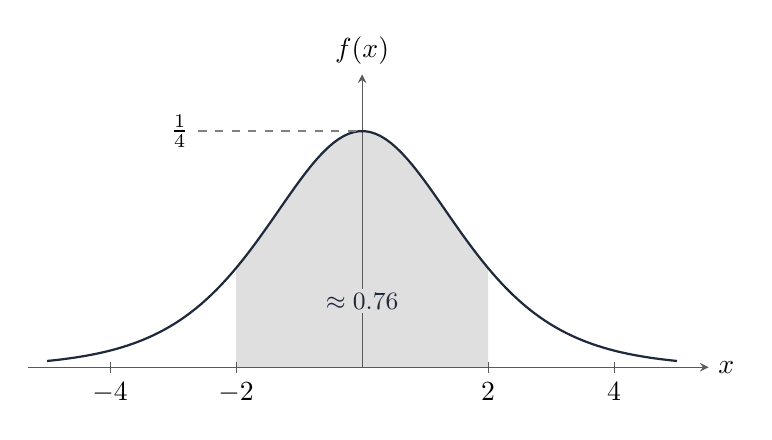
\begin{tikzpicture}[x=0.8cm, y=12cm, >=stealth]
  \fill[gray!25, domain=-2:2, samples=60]
    (-2,0) -- plot (\x, {1/((exp(\x/2)+exp(-\x/2))^2)}) -- (2,0) -- cycle;
  \draw[->, gray!70!black] (-5.3,0) -- (5.5,0) node[right, black] {$x$};
  \draw[->, gray!70!black] (0,0) -- (0,0.31) node[above, black] {$f(x)$};
  \draw[ink, thick, domain=-5:5, samples=120]
    plot (\x, {1/((exp(\x/2)+exp(-\x/2))^2)});
  \foreach \x in {-4,-2,2,4}
    \draw[gray!70!black] (\x,0.006) -- (\x,-0.006) node[below, black] {$\x$};
  \draw[gray, dashed] (-2.6,0.25) -- (0,0.25);
  \node[left] at (-2.6,0.25) {$\tfrac14$};
  \node[ink, fill=gray!25, inner sep=1.5pt] at (0,0.07) {\small $\approx 0.76$};
\end{tikzpicture}
\end{center}
\medskip
The shaded area is $P(-2 < X < 2)$. Since we already have $F$ as an antiderivative,
\medskip
\[
P(-2 < X < 2) = F(2) - F(-2) = \frac{e^{2}}{1 + e^{2}} - \frac{e^{-2}}{1 + e^{-2}} \approx 0.881 - 0.119 = 0.76.
\]
\bigskip

\textbf{Without knowing $F$.} Substitute $u = 1 + e^{x}$, so $du = e^{x}\,dx$, and the limits $x = \pm 2$ become $u = 1 + e^{\pm 2}$:
\medskip
\[
\int_{-2}^{2} \frac{e^{x}}{(1 + e^{x})^{2}}\,dx
= \int_{1 + e^{-2}}^{1 + e^{2}} \frac{1}{u^{2}}\,du
= \left[-\frac{1}{u}\right]_{1 + e^{-2}}^{1 + e^{2}}
\approx 0.76.
\]
\end{solution}

\bigskip

\begin{example}[Rayleigh distribution]\label{ex:rayleigh}
The \textbf{Rayleigh} distribution has CDF
\medskip
\[
F(x) = 1 - e^{-x^{2}/2}, \qquad x > 0.
\]
\medskip
Find the PDF and $P(X > 2)$.
\end{example}

\medskip

\begin{solution}
By the chain rule,
\medskip
\[
f(x) = F'(x) = -e^{-x^{2}/2} \cdot (-x) = x\,e^{-x^{2}/2}, \qquad x > 0.
\]
\medskip
We could integrate $f$ from $2$ to $\infty$ with $u = x^{2}/2$, but $F$ already does the work:
\medskip
\[
P(X > 2) = \int_{2}^{\infty} x\,e^{-x^{2}/2}\,dx = 1 - F(2) = e^{-2} \approx 0.135.
\]
\end{solution}

\bigskip

\begin{definition}[Expectation of a Continuous r.v.]\label{def:contE}
The \textbf{expected value} of a continuous r.v.\ $X$ with PDF $f$ is
\medskip
\[
\E(X) = \int_{-\infty}^{\infty} x\,f(x)\,dx,
\]
\medskip
as long as $\int_{-\infty}^{\infty} |x|\,f(x)\,dx < \infty$. In practice we only integrate over the support, since $f = 0$ elsewhere.
\end{definition}

\bigskip

\begin{intuition}
Same idea as the discrete case: replace the sum with an integral and the PMF with the PDF. $\E(X)$ is still the balancing point of the distribution. The units work out too: $x\,f(x)\,dx$ has units cm $\cdot$ cm$^{-1}$ $\cdot$ cm $=$ cm.
\end{intuition}

\bigskip

\begin{example}[Mean of the $x^{2}$ density]\label{ex:cx2mean}
Find $\E(X)$ for the PDF $f(x) = \tfrac{3}{8}x^{2}$ on $[0, 2]$ from Example~\ref{ex:cx2}.
\end{example}

\medskip

\begin{solution}
\medskip
\[
\E(X) = \int_{0}^{2} x \cdot \frac{3}{8}x^{2}\,dx = \frac{3}{8} \cdot \frac{x^{4}}{4}\bigg|_{0}^{2} = \frac{3}{8} \cdot 4 = \frac{3}{2}.
\]
\medskip
The mean is above the midpoint $1$, which makes sense since the density piles up toward $2$.
\end{solution}

\bigskip

\begin{example}[Mean of the Logistic, by symmetry]
Show that $X \sim$ Logistic has $\E(X) = 0$.
\end{example}

\medskip

\begin{solution}
The PDF is symmetric about $0$: multiplying top and bottom by $e^{2x}$,
\medskip
\[
f(-x) = \frac{e^{-x}}{(1 + e^{-x})^{2}} = \frac{e^{x}}{(e^{x} + 1)^{2}} = f(x).
\]
\medskip
The tails of $f$ shrink like $e^{-|x|}$, so $\int |x|\,f(x)\,dx < \infty$ and the mean exists. For a symmetric density, the contributions $x\,f(x)$ and $(-x)\,f(-x)$ cancel, so $\E(X) = 0$.
\end{solution}

\bigskip

\begin{theorem}[LOTUS, Continuous]\label{thm:lotuscont}
If $X$ is a continuous r.v.\ with PDF $f$ and $g : \mathbb{R} \to \mathbb{R}$, then
\medskip
\[
\E\bigl(g(X)\bigr) = \int_{-\infty}^{\infty} g(x)\,f(x)\,dx.
\]
\end{theorem}

\medskip

\begin{proof}
We prove the case where $g$ is strictly increasing and differentiable. Let $Y = g(X)$, and let $(a, b)$ be the range of $g$ (possibly infinite). Since $g$ is strictly increasing, $g^{-1}$ exists and is strictly increasing too, so for $y \in (a, b)$,
\medskip
\begin{align*}
F_Y(y)
  &= P(g(X) \le y) = P\bigl(X \le g^{-1}(y)\bigr) = F_X\bigl(g^{-1}(y)\bigr).
  && \by{$g$ increasing}
\end{align*}
\medskip
Differentiating with the chain rule,
\medskip
\[
f_Y(y) = f_X\bigl(g^{-1}(y)\bigr) \cdot \frac{d}{dy}\, g^{-1}(y), \qquad a < y < b,
\]
\medskip
and $f_Y(y) = 0$ outside $(a, b)$. So
\medskip
\[
\E(Y) = \int_{a}^{b} y\, f_X\bigl(g^{-1}(y)\bigr) \frac{d}{dy}\, g^{-1}(y)\,dy.
\]
\medskip
Now substitute $x = g^{-1}(y)$. Then $y = g(x)$, $dx = \frac{d}{dy}g^{-1}(y)\,dy$, and as $y$ runs from $a$ to $b$, $x$ runs from $-\infty$ to $\infty$:
\medskip
\[
\E\bigl(g(X)\bigr) = \int_{-\infty}^{\infty} g(x)\,f_X(x)\,dx.
\]
\medskip
The general case (any $g$) holds too, but needs more machinery.
\end{proof}

\bigskip

\begin{remark}
Variance is defined exactly as before, $\Var(X) = \E\bigl[(X - \E X)^{2}\bigr]$, and the shortcut $\Var(X) = \E(X^{2}) - (\E X)^{2}$ still holds. With continuous LOTUS, $\E(X^{2}) = \int x^{2} f(x)\,dx$.
\end{remark}

\bigskip

\begin{example}[Variance of the $x^{2}$ density]
Find $\Var(X)$ for $f(x) = \tfrac{3}{8}x^{2}$ on $[0, 2]$.
\end{example}

\medskip

\begin{solution}
By continuous LOTUS with $g(x) = x^{2}$,
\medskip
\[
\E(X^{2}) = \int_{0}^{2} x^{2} \cdot \frac{3}{8}x^{2}\,dx = \frac{3}{8} \cdot \frac{x^{5}}{5}\bigg|_{0}^{2} = \frac{3}{8} \cdot \frac{32}{5} = \frac{12}{5}.
\]
\medskip
Using $\E(X) = \tfrac{3}{2}$ from Example~\ref{ex:cx2mean},
\medskip
\[
\Var(X) = \E(X^{2}) - (\E X)^{2} = \frac{12}{5} - \frac{9}{4} = \frac{48 - 45}{20} = \frac{3}{20}.
\]
\end{solution}

\medskip

% ============================================================
\subsection{Uniform}
% ============================================================

A uniform r.v.\ on the interval $(a, b)$ is a completely random number between $a$ and $b$.

\begin{definition}[Uniform Distribution]\label{def:unif}
  A continuous r.v.\ $U$ has the \textbf{Uniform distribution} on $(a, b)$, written $U \sim \Unif(a, b)$, if its PDF is
  \[
    f(x) =
    \begin{cases}
      \dfrac{1}{b - a}, & a < x < b, \\[0.6em]
      0,                & \text{otherwise}.
    \end{cases}
  \]
  The CDF is the accumulated area under the PDF:
  \[
    F(x) =
    \begin{cases}
      0,                  & x \le a,     \\[0.2em]
      \dfrac{x - a}{b - a}, & a < x < b, \\[0.6em]
      1,                  & x \ge b.
    \end{cases}
  \]
  $\Unif(0, 1)$ is called the \textbf{standard Uniform} distribution.
\end{definition}

\begin{center}
  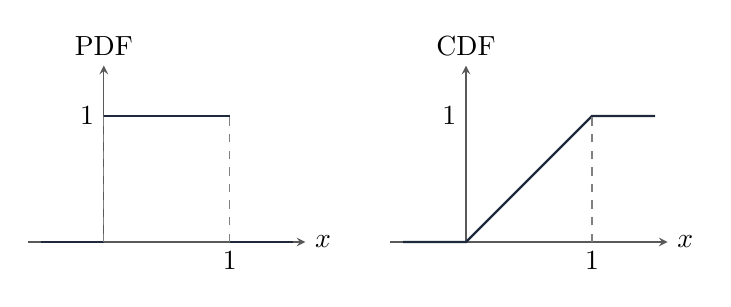
\begin{tikzpicture}[x=1.6cm, y=1.6cm, >=stealth]
    % PDF
    \begin{scope}
      \draw[->, gray!70!black] (-0.6,0) -- (1.6,0) node[right, black] {$x$};
      \draw[->, gray!70!black] (0,0) -- (0,1.4) node[above, black] {PDF};
      \draw[ink, thick] (-0.5,0) -- (0,0);
      \draw[ink, thick] (0,1) -- (1,1);
      \draw[ink, thick] (1,0) -- (1.5,0);
      \draw[gray, dashed] (0,0) -- (0,1) (1,0) -- (1,1);
      \node[below] at (1,0) {$1$};
      \node[left] at (0,1) {$1$};
    \end{scope}

    % CDF
    \begin{scope}[xshift=4.6cm]
      \draw[->, gray!70!black] (-0.6,0) -- (1.6,0) node[right, black] {$x$};
      \draw[->, gray!70!black] (0,0) -- (0,1.4) node[above, black] {CDF};
      \draw[ink, thick] (-0.5,0) -- (0,0) -- (1,1) -- (1.5,1);
      \draw[gray, dashed] (1,0) -- (1,1);
      \node[below] at (1,0) {$1$};
      \node[left] at (0,1) {$1$};
    \end{scope}
  \end{tikzpicture}

  {\small $\Unif(0,1)$ PDF (left) and CDF (right).}
\end{center}

\begin{remark}
  For $U \sim \Unif(a, b)$ and any subinterval $(c, d)$ of $(a, b)$,
  \[
    P\bigl(U \in (c, d)\bigr) = \frac{d - c}{b - a},
  \]
  so probability is \emph{proportional to length}. For $\Unif(0, 1)$, probability \emph{is} length.
\end{remark}

\begin{proposition}[Conditioning a Uniform]\label{prop:unifcond}
  Let $U \sim \Unif(a, b)$ and let $(c, d)$ be a subinterval of $(a, b)$. Then the conditional distribution of $U$ given $U \in (c, d)$ is $\Unif(c, d)$.
\end{proposition}

\begin{proof}
  For $c < u < d$,
  \begin{align*}
    P\bigl(U \le u \mid U \in (c, d)\bigr)
      &= \frac{P\bigl(U \le u,\; c < U < d\bigr)}{P\bigl(U \in (c, d)\bigr)}
      && \by{def.\ of cond.\ prob.} \\[0.4em]
      &= \frac{P\bigl(U \in (c, u]\bigr)}{P\bigl(U \in (c, d)\bigr)}
      && \by{both events at once} \\[0.4em]
      &= \frac{(u - c)/(b - a)}{(d - c)/(b - a)}
       = \frac{u - c}{d - c},
      && \by{prob.\ $\propto$ length}
  \end{align*}
  which is the $\Unif(c, d)$ CDF.
\end{proof}

\begin{example}[Zooming in on a Uniform]
  Let $U \sim \Unif(0, 1)$. Find $P(0.2 < U < 0.6)$, and then $P(U < 0.5 \mid 0.2 < U < 0.6)$.
\end{example}

\begin{solution}
  Probability is length, so $P(0.2 < U < 0.6) = 0.4$. Given $U \in (0.2, 0.6)$, $U \sim \Unif(0.2, 0.6)$ by Proposition~\ref{prop:unifcond}, so
  \[
    P(U < 0.5 \mid 0.2 < U < 0.6) = \frac{0.5 - 0.2}{0.6 - 0.2} = \frac{0.3}{0.4} = \frac{3}{4}.
  \]
\end{solution}

\begin{theorem}[Uniform Mean and Variance]\label{thm:unifEV}
  If $U \sim \Unif(a, b)$, then
  \[
    \E(U) = \frac{a + b}{2},
    \qquad
    \Var(U) = \frac{(b - a)^{2}}{12}.
  \]
\end{theorem}

\begin{proof}
  The mean is the midpoint, as expected since the PDF is flat:
  \[
    \E(U) = \int_{a}^{b} x \cdot \frac{1}{b - a}\,dx = \frac{1}{b - a}\left(\frac{b^{2}}{2} - \frac{a^{2}}{2}\right) = \frac{a + b}{2}.
  \]
  For the variance, first find $\E(U^{2})$ with continuous LOTUS:
  \begin{align*}
    \E(U^{2})
      &= \int_{a}^{b} x^{2} \cdot \frac{1}{b - a}\,dx
       = \frac{1}{3} \cdot \frac{b^{3} - a^{3}}{b - a}
      && \by{LOTUS} \\[0.4em]
      &= \frac{a^{2} + ab + b^{2}}{3}.
      && \by{$b^{3} - a^{3} = (b - a)(a^{2} + ab + b^{2})$}
  \end{align*}
  Then
  \begin{align*}
    \Var(U)
      &= \frac{a^{2} + ab + b^{2}}{3} - \frac{(a + b)^{2}}{4}
       = \frac{4a^{2} + 4ab + 4b^{2} - 3a^{2} - 6ab - 3b^{2}}{12}
      && \by{common denominator} \\[0.4em]
      &= \frac{a^{2} - 2ab + b^{2}}{12}
       = \frac{(b - a)^{2}}{12}.
  \end{align*}
\end{proof}

\begin{definition}[Location-Scale Transformation]\label{def:locscale}
  Let $X$ be an r.v.\ and $Y = \sigma X + \mu$, where $\sigma$ and $\mu$ are constants with $\sigma > 0$. We say $Y$ is obtained from $X$ by a \textbf{location-scale transformation}: $\mu$ controls how the location is changed (shift) and $\sigma$ controls how the scale is changed (stretch).
\end{definition}

\begin{example}[Uniform mean and variance, the easy way]
  Use a location-scale transformation to get Theorem~\ref{thm:unifEV} without the algebra.
\end{example}

\begin{solution}
  Start with $U \sim \Unif(0, 1)$, whose PDF is $1$ on $(0, 1)$:
  \[
    \E(U) = \int_{0}^{1} x\,dx = \frac{1}{2},
    \qquad
    \E(U^{2}) = \int_{0}^{1} x^{2}\,dx = \frac{1}{3},
    \qquad
    \Var(U) = \frac{1}{3} - \frac{1}{4} = \frac{1}{12}.
  \]
  To turn $U$ into a general $\Unif(a, b)$ r.v., stretch the support from length $1$ to length $b - a$ (multiply by $b - a$, giving $\Unif(0, b - a)$), then shift it to start at $a$:
  \[
    \tilde{U} = a + (b - a)U \sim \Unif(a, b).
  \]
  Now linearity and the properties of variance do the work:
  \begin{align*}
    \E(\tilde{U}) &= a + (b - a)\,\E(U) = a + \frac{b - a}{2} = \frac{a + b}{2},
      && \by{linearity} \\[0.4em]
    \Var(\tilde{U}) &= (b - a)^{2}\,\Var(U) = \frac{(b - a)^{2}}{12}.
      && \by{shift drops out, scale comes out squared}
  \end{align*}
\end{solution}

% ============================================================
\subsection{Universality of the Uniform}
% ============================================================

Given a $\Unif(0, 1)$ r.v., we can construct an r.v.\ with any continuous distribution we want. Conversely, given an r.v.\ with any continuous distribution, we can create a $\Unif(0, 1)$ r.v. We call this the \textbf{universality of the Uniform}, because it tells us the Uniform is a universal starting point for building r.v.s with other distributions. (It's also called the probability integral transform, inverse transform sampling, or the quantile transformation.)

\begin{theorem}[Universality of the Uniform]\label{thm:universality}
  Let $F$ be a CDF that is continuous and strictly increasing on the support, so $F^{-1}$ exists, and let $U \sim \Unif(0, 1)$.
  \begin{enumerate}
    \item If $X = F^{-1}(U)$, then $X$ has CDF $F$.
    \item If $X$ has CDF $F$, then $F(X) \sim \Unif(0, 1)$.
  \end{enumerate}
\end{theorem}

\begin{proof}
  (1) For any $x$,
  \begin{align*}
    P(X \le x)
      &= P\bigl(F^{-1}(U) \le x\bigr)
       = P\bigl(U \le F(x)\bigr)
      && \by{apply $F$ to both sides; $F$ increasing} \\[0.4em]
      &= F(x).
      && \by{$P(U \le u) = u$ for $u \in (0, 1)$}
  \end{align*}
  (2) For $0 < u < 1$,
  \[
    P\bigl(F(X) \le u\bigr) = P\bigl(X \le F^{-1}(u)\bigr) = F\bigl(F^{-1}(u)\bigr) = u,
  \]
  which is the $\Unif(0, 1)$ CDF.
\end{proof}

\begin{intuition}
  Recipe for part (1): take the CDF you're interested in, take its inverse, and plug in the Uniform. $U$ picks a random height between $0$ and $1$ on the CDF's vertical axis, and $F^{-1}$ reads off which $x$ is at that height. Steep parts of $F$ (where the PDF is big) cover lots of heights over a short stretch of $x$, so $X$ lands there more often.
\end{intuition}

\begin{example}[Simulating a Logistic]
  Using one $U \sim \Unif(0, 1)$, construct an r.v.\ with the Logistic distribution from Example~\ref{ex:logistic}.
\end{example}

\begin{solution}
  Invert $F(x) = \frac{e^{x}}{1 + e^{x}}$ by solving $u = \frac{e^{x}}{1 + e^{x}}$ for $x$:
  \[
    u(1 + e^{x}) = e^{x}
    \;\Longrightarrow\;
    e^{x} = \frac{u}{1 - u}
    \;\Longrightarrow\;
    F^{-1}(u) = \ln\!\left(\frac{u}{1 - u}\right).
  \]
  So by Theorem~\ref{thm:universality}, $X = \ln\!\left(\frac{U}{1 - U}\right) \sim$ Logistic.
\end{solution}

% ============================================================
\subsection{Normal}
% ============================================================

The Normal is a continuous distribution with a bell-shaped PDF. Once we have the \emph{standard} Normal, we'll be able to get any Normal distribution we want by shifting and scaling.

\begin{definition}[Standard Normal Distribution]\label{def:stdnormal}
  A continuous r.v.\ $Z$ has the \textbf{standard Normal distribution}, written $Z \sim \Norm(0, 1)$, if its PDF is
  \[
    \varphi(z) = \frac{1}{\sqrt{2\pi}}\, e^{-z^{2}/2}, \qquad -\infty < z < \infty.
  \]
  The standard Normal CDF $\Phi$ is the accumulated area under the PDF:
  \[
    \Phi(z) = \int_{-\infty}^{z} \varphi(t)\,dt = \int_{-\infty}^{z} \frac{1}{\sqrt{2\pi}}\, e^{-t^{2}/2}\,dt.
  \]
\end{definition}

\begin{remark}
  There is no closed-form expression for the antiderivative of $\varphi$: we can't write $\Phi$ in terms of elementary functions. So $\Phi$ is just \emph{defined} as this integral, and in practice we get its values from software or a table.
\end{remark}

\begin{center}
  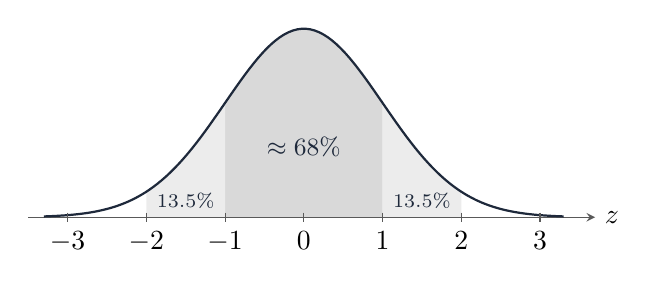
\begin{tikzpicture}[x=1cm, y=6cm, >=stealth]
    \fill[gray!30, domain=-1:1, samples=60]
      (-1,0) -- plot (\x, {exp(-\x*\x/2)/sqrt(2*pi)}) -- (1,0) -- cycle;
    \fill[gray!15, domain=-2:-1, samples=40]
      (-2,0) -- plot (\x, {exp(-\x*\x/2)/sqrt(2*pi)}) -- (-1,0) -- cycle;
    \fill[gray!15, domain=1:2, samples=40]
      (1,0) -- plot (\x, {exp(-\x*\x/2)/sqrt(2*pi)}) -- (2,0) -- cycle;
    \draw[->, gray!70!black] (-3.5,0) -- (3.7,0) node[right, black] {$z$};
    \draw[ink, thick, domain=-3.3:3.3, samples=120]
      plot (\x, {exp(-\x*\x/2)/sqrt(2*pi)});
    \foreach \x in {-3,-2,-1,0,1,2,3}
      \draw[gray!70!black] (\x,0.01) -- (\x,-0.01) node[below, black] {$\x$};
    \node[ink] at (0,0.15) {\small $\approx 68\%$};
    \node[ink] at (-1.5,0.035) {\scriptsize $13.5\%$};
    \node[ink] at (1.5,0.035) {\scriptsize $13.5\%$};
  \end{tikzpicture}

  {\small Standard Normal PDF $\varphi$. Dark: within $1$ SD of the mean; dark + light: within $2$ SDs ($\approx 95\%$).}
\end{center}

\begin{formula}[Symmetry properties of the standard Normal]
  \begin{enumerate}
    \item \textbf{Symmetry of the PDF:} $\varphi(z) = \varphi(-z)$.
    \item \textbf{Symmetry of tail areas:} the area to the left of $-z$ equals the area to the right of $z$, i.e.\ $P(Z \le -z) = P(Z \ge z)$, so
    \[
      \Phi(z) = 1 - \Phi(-z) \quad \text{for all } z.
    \]
    \item \textbf{Symmetry of $Z$ and $-Z$:} if $Z \sim \Norm(0, 1)$, then $-Z \sim \Norm(0, 1)$ as well.
  \end{enumerate}
\end{formula}

\begin{proof}
  (1) $z$ only appears as $z^{2}$. (2) Substitute $u = -t$ and use that the PDF integrates to $1$:
  \[
    \Phi(-z) = \int_{-\infty}^{-z} \varphi(t)\,dt = \int_{z}^{\infty} \varphi(u)\,du = 1 - \int_{-\infty}^{z} \varphi(u)\,du = 1 - \Phi(z).
  \]
  (3) $P(-Z \le z) = P(Z \ge -z) = 1 - \Phi(-z) = \Phi(z)$, using (2). So $-Z$ has CDF $\Phi$.
\end{proof}

\begin{theorem}[$\varphi$ is a Valid PDF]\label{thm:phivalid}
  $\displaystyle\int_{-\infty}^{\infty} e^{-z^{2}/2}\,dz = \sqrt{2\pi}$, so $\varphi$ integrates to $1$.
\end{theorem}

\begin{proof}
  We can't integrate $e^{-z^{2}/2}$ directly, so we square the integral and switch to polar coordinates. Since $z$ is a dummy variable, call it $x$ in one copy and $y$ in the other:
  \begin{align*}
    \left(\int_{-\infty}^{\infty} e^{-z^{2}/2}\,dz\right)^{2}
      &= \left(\int_{-\infty}^{\infty} e^{-x^{2}/2}\,dx\right)\left(\int_{-\infty}^{\infty} e^{-y^{2}/2}\,dy\right)
      && \by{rename dummy variables} \\[0.4em]
      &= \int_{-\infty}^{\infty}\int_{-\infty}^{\infty} e^{-(x^{2} + y^{2})/2}\,dx\,dy
      && \by{combine into a double integral} \\[0.4em]
      &= \int_{0}^{2\pi}\int_{0}^{\infty} e^{-r^{2}/2}\, r\,dr\,d\theta
      && \by{polar; extra $r$ is the Jacobian} \\[0.4em]
      &= \int_{0}^{2\pi}\left(\int_{0}^{\infty} e^{-u}\,du\right) d\theta
      && \by{$u = r^{2}/2$, $du = r\,dr$} \\[0.4em]
      &= \int_{0}^{2\pi} 1\,d\theta = 2\pi.
  \end{align*}
  Taking square roots, the integral is $\sqrt{2\pi}$.
\end{proof}

\begin{theorem}[Standard Normal Mean and Variance]\label{thm:stdnormalEV}
  If $Z \sim \Norm(0, 1)$, then $\E(Z) = 0$ and $\Var(Z) = 1$.
\end{theorem}

\begin{proof}
  \textbf{Mean.} $g(z) = z\,e^{-z^{2}/2}$ is an odd function ($g(-z) = -g(z)$), and the integral of an odd function over a symmetric range is $0$:
  \[
    \E(Z) = \frac{1}{\sqrt{2\pi}} \int_{-\infty}^{\infty} z\, e^{-z^{2}/2}\,dz = 0.
  \]
  \textbf{Variance.} Since $\E(Z) = 0$, $\Var(Z) = \E(Z^{2})$. The integrand $z^{2}e^{-z^{2}/2}$ is even, so
  \begin{align*}
    \Var(Z)
      &= \frac{1}{\sqrt{2\pi}} \int_{-\infty}^{\infty} z^{2} e^{-z^{2}/2}\,dz
       = \frac{2}{\sqrt{2\pi}} \int_{0}^{\infty} z^{2} e^{-z^{2}/2}\,dz
      && \by{LOTUS; even function} \\[0.4em]
      &= \frac{2}{\sqrt{2\pi}} \left( \Bigl[-z\,e^{-z^{2}/2}\Bigr]_{0}^{\infty} + \int_{0}^{\infty} e^{-z^{2}/2}\,dz \right)
      && \by{parts: $u = z$, $dv = z e^{-z^{2}/2}dz$} \\[0.4em]
      &= \frac{2}{\sqrt{2\pi}} \left( 0 + \frac{\sqrt{2\pi}}{2} \right) = 1.
      && \by{Thm~\ref{thm:phivalid}, half the area}
  \end{align*}
\end{proof}

\begin{definition}[Normal Distribution]\label{def:normal}
  If $Z \sim \Norm(0, 1)$, then
  \[
    X = \mu + \sigma Z
  \]
  has the \textbf{Normal distribution} with mean $\mu$ and variance $\sigma^{2}$, for any real $\mu$ and $\sigma > 0$. We write $X \sim \Norm(\mu, \sigma^{2})$.
\end{definition}

\begin{remark}
  This is a location-scale transformation of $Z$, so by linearity and the variance properties, $\E(X) = \mu + \sigma \cdot 0 = \mu$ and $\Var(X) = \sigma^{2} \cdot 1 = \sigma^{2}$. Going the other way, \textbf{standardization}: if $X \sim \Norm(\mu, \sigma^{2})$ then
  \[
    Z = \frac{X - \mu}{\sigma} \sim \Norm(0, 1).
  \]
\end{remark}

\begin{theorem}[Normal CDF and PDF]\label{thm:normalcdf}
  Let $X \sim \Norm(\mu, \sigma^{2})$. Then the CDF and PDF of $X$ are
  \[
    F(x) = \Phi\!\left(\frac{x - \mu}{\sigma}\right),
    \qquad
    f(x) = \varphi\!\left(\frac{x - \mu}{\sigma}\right) \frac{1}{\sigma} = \frac{1}{\sqrt{2\pi}\,\sigma} \exp\!\left(-\frac{(x - \mu)^{2}}{2\sigma^{2}}\right).
  \]
\end{theorem}

\begin{proof}
  Standardize inside the probability:
  \begin{align*}
    F(x) = P(X \le x)
      &= P\!\left(\frac{X - \mu}{\sigma} \le \frac{x - \mu}{\sigma}\right)
      && \by{same event, $\sigma > 0$} \\[0.4em]
      &= \Phi\!\left(\frac{x - \mu}{\sigma}\right).
      && \by{standardized $X$ is $\Norm(0,1)$}
  \end{align*}
  Differentiating with the chain rule gives $f(x) = \varphi\!\left(\frac{x - \mu}{\sigma}\right)\cdot\frac{1}{\sigma}$, and plugging in the formula for $\varphi$ gives the last form.
\end{proof}

\begin{formula}[68--95--99.7\% rule]
  If $X \sim \Norm(\mu, \sigma^{2})$, then
  \[
    P(|X - \mu| < \sigma) \approx 0.68,
    \qquad
    P(|X - \mu| < 2\sigma) \approx 0.95,
    \qquad
    P(|X - \mu| < 3\sigma) \approx 0.997.
  \]
  That is, the chance of falling within $1$, $2$, $3$ SDs of the mean.
\end{formula}

\begin{example}[Using the 68--95--99.7 rule]\label{ex:normalrule}
  Let $X \sim \Norm(-1, 4)$. Approximate $P(|X| < 3)$.
\end{example}

\begin{solution}
  Here $\mu = -1$ and $\sigma = 2$. $|X| < 3$ is the same as $-3 < X < 3$. Standardize with $Z = \frac{X - (-1)}{2}$:
  \begin{align*}
    P(-3 < X < 3)
      &= P\!\left(\frac{-3 - (-1)}{2} < \frac{X - (-1)}{2} < \frac{3 - (-1)}{2}\right)
      && \by{standardize} \\[0.4em]
      &= P(-1 < Z < 2).
  \end{align*}
  The rule says $P(-1 < Z < 1) \approx 0.68$ and $P(-2 < Z < 2) \approx 0.95$, so the two bands between $1$ and $2$ SDs hold $0.95 - 0.68 = 0.27$ together, and by symmetry $P(1 < Z < 2) \approx 0.27/2$. So
  \[
    P(-1 < Z < 2) = P(-1 < Z < 1) + P(1 < Z < 2) \approx 0.68 + 0.135 = 0.815.
  \]
  The exact value is $\Phi(2) - \Phi(-1) \approx 0.8186$, so the rule does well.
\end{solution}

\begin{example}[Folded Normal]\label{ex:foldednormal}
  Let $Y = |Z|$ with $Z \sim \Norm(0, 1)$. Find (a) $\E(Y)$, (b) $\Var(Y)$, (c) the CDF and PDF of $Y$.
\end{example}

\begin{solution}
  (a) By LOTUS, and since $|z|\varphi(z)$ is even,
  \begin{align*}
    \E(Y)
      &= \int_{-\infty}^{\infty} |z|\, \frac{1}{\sqrt{2\pi}} e^{-z^{2}/2}\,dz
       = \frac{2}{\sqrt{2\pi}} \int_{0}^{\infty} z\, e^{-z^{2}/2}\,dz
      && \by{even function} \\[0.4em]
      &= \frac{2}{\sqrt{2\pi}} \Bigl[-e^{-z^{2}/2}\Bigr]_{0}^{\infty}
       = \frac{2}{\sqrt{2\pi}}
       = \sqrt{\frac{2}{\pi}} \approx 0.80.
  \end{align*}
  (b) $\E(Y^{2}) = \E(Z^{2}) = \Var(Z) = 1$, so
  \[
    \Var(Y) = \E(Y^{2}) - (\E Y)^{2} = 1 - \frac{2}{\pi} \approx 0.36.
  \]
  (c) For $y \ge 0$,
  \[
    F_Y(y) = P(|Z| \le y) = P(-y \le Z \le y) = \Phi(y) - \Phi(-y) = 2\Phi(y) - 1,
  \]
  using $\Phi(-y) = 1 - \Phi(y)$, and $F_Y(y) = 0$ for $y < 0$. Differentiating,
  \[
    f_Y(y) = 2\varphi(y) = \sqrt{\frac{2}{\pi}}\, e^{-y^{2}/2}, \qquad y > 0.
  \]
\end{solution}

% ============================================================
\subsection{Exponential}
% ============================================================

The Exponential is the continuous counterpart of the Geometric. A Geometric r.v.\ counts the number of failures before the first success in a sequence of Bernoulli trials. With the Exponential, we're waiting for a success in \emph{continuous time}, where successes arrive at a rate of $\lambda$ per unit of time. The average number of successes in a time interval of length $t$ is $\lambda t$, though the actual number varies randomly. An Exponential r.v.\ represents the waiting time until the first arrival.

\begin{definition}[Exponential Distribution]\label{def:expo}
  A continuous r.v.\ $X$ has the \textbf{Exponential distribution} with parameter (rate) $\lambda > 0$, written $X \sim \Expo(\lambda)$, if its PDF is
  \[
    f(x) = \lambda e^{-\lambda x}, \qquad x > 0.
  \]
  This is valid since $\int_{0}^{\infty} \lambda e^{-\lambda x}\,dx = 1$. The CDF is
  \[
    F(x) = \int_{0}^{x} \lambda e^{-\lambda t}\,dt = 1 - e^{-\lambda x}, \qquad x > 0.
  \]
\end{definition}

\begin{proposition}[Scaling to $\Expo(1)$]\label{prop:exposcale}
  If $X \sim \Expo(\lambda)$, then $Y = \lambda X \sim \Expo(1)$.
\end{proposition}

\begin{proof}
  For $y > 0$,
  \[
    P(Y \le y) = P\!\left(X \le \frac{y}{\lambda}\right) = 1 - e^{-\lambda \cdot y/\lambda} = 1 - e^{-y},
  \]
  which is the $\Expo(1)$ CDF.
\end{proof}

\begin{theorem}[Exponential Mean and Variance]\label{thm:expoEV}
  If $X \sim \Expo(\lambda)$, then
  \[
    \E(X) = \frac{1}{\lambda},
    \qquad
    \Var(X) = \frac{1}{\lambda^{2}}.
  \]
\end{theorem}

\begin{proof}
  First do $Y \sim \Expo(1)$, using integration by parts each time.

  \textbf{First moment.} With $u = y$, $dv = e^{-y}dy$ (so $du = dy$, $v = -e^{-y}$):
  \[
    \E(Y) = \int_{0}^{\infty} y\, e^{-y}\,dy = \Bigl[-y\,e^{-y}\Bigr]_{0}^{\infty} + \int_{0}^{\infty} e^{-y}\,dy = 0 + 1 = 1.
  \]
  \textbf{Second moment.} With $u = y^{2}$, $dv = e^{-y}dy$:
  \[
    \E(Y^{2}) = \int_{0}^{\infty} y^{2} e^{-y}\,dy = \Bigl[-y^{2} e^{-y}\Bigr]_{0}^{\infty} + 2\int_{0}^{\infty} y\, e^{-y}\,dy = 0 + 2\,\E(Y) = 2,
  \]
  so $\Var(Y) = 2 - 1^{2} = 1$.

  \textbf{General $\lambda$.} By Proposition~\ref{prop:exposcale}, $X = Y/\lambda$ with $Y \sim \Expo(1)$, so
  \[
    \E(X) = \frac{\E(Y)}{\lambda} = \frac{1}{\lambda},
    \qquad
    \Var(X) = \frac{\Var(Y)}{\lambda^{2}} = \frac{1}{\lambda^{2}}.
  \]
\end{proof}

\begin{pitfall}
  $\lambda$ is a \emph{rate}, not a mean. If buses come on average every $10$ minutes, then $\lambda = 1/10$ per minute, not $10$. (Some books parametrize the Exponential by its mean instead, so always check.)
\end{pitfall}

\begin{definition}[Memoryless Property]\label{def:memoryless}
  A continuous distribution on $(0, \infty)$ is \textbf{memoryless} if, for $X$ with that distribution,
  \[
    P(X \ge s + t \mid X \ge s) = P(X \ge t) \quad \text{for all } s, t \ge 0.
  \]
  Think of $X$ as a waiting time (e.g.\ for a phone call): if you've already waited $s$ minutes, the chance of waiting at least $t$ \emph{more} minutes is the same as if you'd just started.
\end{definition}

\begin{theorem}[The Exponential is Memoryless]\label{thm:expomemoryless}
  If $X \sim \Expo(\lambda)$, then $X$ has the memoryless property.
\end{theorem}

\begin{proof}
  Here $P(X \ge s) = 1 - P(X \le s) = e^{-\lambda s}$. Then
  \begin{align*}
    P(X \ge s + t \mid X \ge s)
      &= \frac{P(X \ge s + t,\; X \ge s)}{P(X \ge s)}
      && \by{def.\ of cond.\ prob.} \\[0.4em]
      &= \frac{P(X \ge s + t)}{P(X \ge s)}
      && \by{$X \ge s$ is redundant} \\[0.4em]
      &= \frac{e^{-\lambda(s + t)}}{e^{-\lambda s}} = e^{-\lambda t} = P(X \ge t).
  \end{align*}
\end{proof}

\begin{example}[Waiting for a bus]
  Bus arrivals at a stop follow a rate of one every $10$ minutes on average, so your wait is $X \sim \Expo(1/10)$ in minutes. You've already waited $10$ minutes. What's the probability you wait more than $15$ minutes in total?
\end{example}

\begin{solution}
  By memorylessness, having waited $10$ minutes changes nothing:
  \[
    P(X > 15 \mid X > 10) = P(X > 5) = e^{-5/10} = e^{-0.5} \approx 0.61.
  \]
  Your expected \emph{remaining} wait is still $1/\lambda = 10$ minutes, no matter how long you've been standing there.
\end{solution}

\begin{theorem}[Memoryless Implies Exponential]\label{thm:memorylessexpo}
  If $X$ is a positive continuous r.v.\ with the memoryless property, then $X \sim \Expo(\lambda)$ for some $\lambda > 0$.
\end{theorem}

\begin{proof}
  Let $F$ be the CDF of $X$ and $G(x) = P(X > x) = 1 - F(x)$. The memoryless property says
  \[
    G(s + t) = G(s)\,G(t) \quad \text{for all } s, t \ge 0.
  \]
  We solve for $G$.
  \begin{itemize}
    \item Taking $s = t$ gives $G(2t) = G(t)^{2}$, then $G(3t) = G(t)^{3}$, and in general $G(kt) = G(t)^{k}$ for positive integers $k$.
    \item Replacing $t$ by $t/k$: $G(t) = G(t/k)^{k}$, so $G(t/k) = G(t)^{1/k}$.
    \item Combining the two: $G\!\left(\frac{m}{n}t\right) = G(t)^{m/n}$ for all positive integers $m, n$, so $G(xt) = G(t)^{x}$ for every positive rational $x$.
    \item Any positive real number is a limit of positive rationals, and $G$ is continuous, so $G(xt) = G(t)^{x}$ for all real $x > 0$.
  \end{itemize}
  Taking $t = 1$: $G(x) = G(1)^{x} = e^{-\lambda x}$, where $\lambda = -\ln G(1)$. Since $X$ is positive and continuous, $0 < G(1) < 1$, so $\lambda > 0$. Then $F(x) = 1 - e^{-\lambda x}$, the $\Expo(\lambda)$ CDF.
\end{proof}




\end{document}